\documentclass{beamer}
%
% Choose how your presentation looks.
%
% For more themes, color themes and font themes, see:
% http://deic.uab.es/~iblanes/beamer_gallery/index_by_theme.html
%
\mode<presentation>
{
  \usetheme{default}      % or try Darmstadt, Madrid, Warsaw, ...
  \usecolortheme{default} % or try albatross, beaver, crane, ...
  \usefonttheme{default}  % or try serif, structurebold, ...
  \setbeamertemplate{navigation symbols}{}
  \setbeamertemplate{caption}[numbered]
  \setbeamertemplate{footline}[frame number]
  \setbeamertemplate{itemize items}[circle]
%   \setbeamertemplate{theorems}[numbered]
  \setbeamercolor*{structure}{bg=white,fg=blue}
  \setbeamerfont{block title}{size=\normalsize}
  \setbeamercolor{bibliography entry author}{fg=black}
  \setbeamercolor{bibliography entry title}{fg=black}
  \setbeamercolor{bibliography entry note}{fg=black}
}

% \newtheorem{proposition}[theorem]{Proposition}
% \theoremstyle{definition}
% \newtheorem{algorithm}[theorem]{Algorithm}
% \newtheorem{idea}[theorem]{Idea}

\usepackage[english]{babel}
\usepackage[utf8]{inputenc}
\usepackage[T1]{fontenc}
\usepackage{nicefrac}
\usepackage{tabularx}
\usepackage{makecell}
% \usepackage{amsmath,amsfonts,amsthm,amssymb,mathrsfs,bbm,mathtools}
% \usepackage{enumitem}
\usepackage{tikz}
% \usetikzlibrary{patterns}
% \usetikzlibrary{intersections}
% \usepackage{pgfplots}
% \usepgfplotslibrary{fillbetween}
% \usepgfplotslibrary{dateplot}
% \usepackage{pgfplotstable}
\usepackage{appendixnumberbeamer}

% \usepackage{booktabs}
% \usepackage[final]{microtype}
% \usepackage{caption}
% \usepackage{amsmath}
% \usepackage{mathtools}
% \usepackage{amsthm,thmtools}
% % \usepackage[nottoc]{tocbibind}
% % \usepackage[ruled]{algorithm2e}
% \usepackage{enumerate}
% \usepackage[italic]{esdiff}
% \usepackage{subcaption}
% \usepackage{ltablex}
% \usepackage{multirow}

\usepackage{pifont}
\newcommand{\cmark}{\text{\ding{51}}}
\newcommand{\xmark}{\text{\ding{55}}}

%--------Pseudocode--------
\usepackage{xcolor,amsmath}
\usepackage{algorithm2e}
\DontPrintSemicolon
% \SetAlgoSkip{bigskip}

% % Define pseudocode formatting
% \renewcommand{\KwSty}[1]{\textnormal{\textcolor{blue!90!black}{\ttfamily\bfseries #1}}\unskip}
% \renewcommand{\ArgSty}[1]{\textnormal{\ttfamily #1}\unskip}
% \SetKwComment{Comment}{\color{green!50!black}// }{}
% \renewcommand{\CommentSty}[1]{\textnormal{\ttfamily\color{green!50!black}#1}\unskip}
% \newcommand{\assign}{\leftarrow}
% % \newcommand{\var}{\texttt}
% \newcommand{\FuncCall}[2]{\texttt{\bfseries #1(#2)}}
% \SetKwProg{Function}{function}{}{}
% \renewcommand{\ProgSty}[1]{\texttt{\bfseries #1}}

% % Settings for pgfplots
% \pgfplotsset{compat=newest}

% \renewcommand\tabularxcolumn[1]{m{#1}}
% \newcolumntype{R}{>{\raggedleft\arraybackslash}X}=

% \def\code#1{\texttt{\frenchspacing#1}}
\def\padding{\vspace{0.5cm}}
\def\spadding{\vspace{0.25cm}}
\def\b{\textcolor{blue}}
\def\r{\textcolor{red}}
\def\o{\textcolor{orange}}
\def\g#1{{\usebeamercolor[fg]{block title example}{#1}}}
\definecolor{softgreen}{RGB}{124,216,23}

% fix for \pause in align
\makeatletter
\let\save@measuring@true\measuring@true
\def\measuring@true{%
  \save@measuring@true
  \def\beamer@sortzero##1{\beamer@ifnextcharospec{\beamer@sortzeroread{##1}}{}}%
  \def\beamer@sortzeroread##1<##2>{}%
  \def\beamer@finalnospec{}%
}
\makeatother

% \DeclarePairedDelimiter{\norm}{\lVert}{\rVert}
\NewDocumentCommand{\follows}{}{\ensuremath{\rightsquigarrow}\hspace{0.5em}}
\newcommand*{\defeq}{\overset{.}{=}}
\newcommand*{\eqdef}{\overset{.}{=}}
\RenewDocumentCommand{\Pr}{om}{Pr\IfValueT{#1}{_{#1}}{}[#2]}
\NewDocumentCommand{\E}{om}{\mathbb{E}\IfValueT{#1}{_{#1}}{}#2}
\RenewDocumentCommand{\O}{m}{\mathcal{O}(#1)}
\NewDocumentCommand{\B}{}{\mathcal{B}}
\NewDocumentCommand{\G}{}{\mathcal{G}}
\NewDocumentCommand{\C}{}{\o{\mathcal{C}}}
\RenewDocumentCommand{\L}{}{\r{\ensuremath{\mathcal{L}_\tau}}}
\NewDocumentCommand{\U}{}{\b{\ensuremath{\mathcal{U}_\tau}}}
\NewDocumentCommand{\pmax}{}{p_\mathrm{max}}
\NewDocumentCommand{\taumax}{}{\ensuremath{\tau_\mathrm{max}}}
\NewDocumentCommand{\var}{m}{\mathrm{var}(#1)}
\NewDocumentCommand{\maxsize}{m}{\mathrm{maxsize}(#1)}
\NewDocumentCommand{\poly}{m}{\mathrm{poly}(#1)}
\NewDocumentCommand{\polylog}{m}{\mathrm{polylog}(#1)}
\NewDocumentCommand{\distr}{}{D}
\NewDocumentCommand{\law}{}{p}
\NewDocumentCommand{\epslaw}{}{\ensuremath{\law^{1-\epsilon}}}
\NewDocumentCommand{\w}{}{\ensuremath{w_\law}}
\NewDocumentCommand{\epsw}{}{\ensuremath{w_{\epslaw}}}
\NewDocumentCommand{\epsalpha}{}{\ensuremath{\alpha_{\law^{1-\epsilon}}}}
\NewDocumentCommand{\epsW}{}{\ensuremath{W_\epsilon}}
\NewDocumentCommand{\compat}{mm}{#1[#2]}

\newcommand<>{\uncoverubrace}[2]{%
  \onslide#3 \underbrace{ \onslide<4->%
  #1%
  \onslide#3 }_{#2} \onslide<4->%
}

\usepackage[sorting=ynt,style=alphabetic]{biblatex}
\addbibresource{sources.bib}

\renewcommand{\footnotesize}{\tiny}

\begin{document}

\title[Deterministic Algorithms for the Lovász Local Lemma]{Deterministic Algorithms \\ for the Lovász Local Lemma\footfullcite{harris2022deterministic}}
\author{Jonas Hübotter and Duri Janett \\ Advised by Yassir Akram}
\date{March 29, 2022}

\begin{frame}
  \titlepage
\end{frame}

% \begin{frame}{Outline}
%  \tableofcontents[subsubsectionstyle=hide,pausesections]
% \end{frame}
% \AtBeginSection[]
%   {
%      \begin{frame}[allowframebreaks]{Plan}
%      \tableofcontents[currentsection, sectionstyle=show/hide, hideothersubsections]
%      \end{frame}
%   }

\section{Introduction}
\subsection{Lovász Local Lemma and the MT Algorithm}
\begin{frame}{Setting}
Distribution $\distr$ over independent $\Sigma$-valued coordinates $X_1, \dots, X_n$.
``Bad-events'' $\B = \{B_1, \dots, B_m\}$, each a boolean function of some subset of coordinates $\var{B_i} \subseteq \{X_1,\dots,X_n\}$ with law $\law$.

\begin{example}[3-SAT]
\begin{columns}
\begin{column}{.3\textwidth}
$\begin{aligned}
B_1 &\defeq f_1(X_1,X_3,X_5) \\
B_2 &\defeq f_2(X_2,X_3,X_6) \\
B_3 &\defeq f_3(X_1,X_5,X_6) \\
B_4 &\defeq f_4(X_2,X_4,X_7)
\end{aligned}$
\end{column}
\begin{column}{.3\textwidth}
\tikzset{every picture/.style={line width=0.75pt}} %set default line width to 0.75pt        

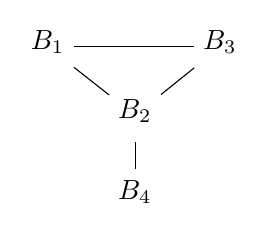
\begin{tikzpicture}[x=0.75pt,y=0.75pt,yscale=-1,xscale=1]
%uncomment if require: \path (0,534); %set diagram left start at 0, and has height of 534


% Text Node
\draw (20,22) node [anchor=north west][inner sep=0.75pt]    {$B_{1}$};
% Text Node
\draw (62,55) node [anchor=north west][inner sep=0.75pt]    {$B_{2}$};
% Text Node
\draw (103,22) node [anchor=north west][inner sep=0.75pt]    {$B_{3}$};
% Text Node
\draw (62,94) node [anchor=north west][inner sep=0.75pt]    {$B_{4}$};
% Connection
\draw    (100,31) -- (42,31) ;
% Connection
\draw    (59,54.18) -- (42,40.82) ;
% Connection
\draw    (84,53.94) -- (100,41.06) ;
% Connection
\draw    (71.5,77) -- (71.5,90) ;

\end{tikzpicture}
\end{column}
\end{columns}
\end{example}\pause

\begin{theorem}[(Symmetric) Lovász Local Lemma]
If for any $i$, $\law(B_i) \leq \pmax$ and $B_i$ affects at most $d$ bad-events, then $e \pmax d \leq 1$ implies $\Pr{\text{all $B_i$ avoided}} > 0$.
\end{theorem}\pause\spadding

For \g{$k$-SAT} and $X_i \sim \text{Unif}(\{0,1\})$, $\law \equiv 2^{-k}$.\par
\follows satisfiable if any variable appears in at most $\nicefrac{2^k}{k e}$ clauses!%\pause\ How to find a satisfying assignment?
\end{frame}

\begin{frame}{Applications}
\begin{example}[k-Coloring]
Choose $C_v \sim \text{Unif}([k])$ independently.\pause\par
$B_{v,c} \defeq \text{``$C_v = c$ and $v$ has neighbor with color $c$''}$.\par
$B_{v,c}$ affects $B_{v',c'}$ iff $v$ and $v'$ have distance $\leq 2$\pause\ \follows $d \leq k \Delta^2$.\pause\par
$p(B_{v,c}) = \frac{1}{k}(\sum_{u \in N(v)} \frac{1}{k}) \leq \frac{\Delta}{k^2}$\pause\ \follows if $e \Delta^3 \leq k$, has $k$-coloring!
\end{example}\pause\padding

More applications:
\begin{enumerate}
    % \item Satisfiability
    \item Defective coloring 
    \item Hypergraph coloring
    \item Strong coloring
    \item Non-repetitive coloring
    \item Finding directed cycles of certain length (see exam, task 2 :))
    \item Independent transversals
\end{enumerate}\pause

\follows algorithmic versions of the Lovász Local Lemma yield automatic algorithms for these problems!
\end{frame}

\begin{frame}{Prior Work}
\begin{algorithm}[H]
    \TitleOfAlgo{MT-Algorithm}
    Draw $X$ from distribution $\distr$\;
    \While{some bad-event is true on $X$}{
        Select any true bad-event $B$\;
        For each $i \in \var{B}$, draw $X_i$ from its distribution in $\distr$\;
    }
\end{algorithm}\pause
\follows converges within expected polynomial time.\footfullcite{moser2010constructive}
\end{frame}

\subsection{Prior Work}
\begin{frame}{Prior Work}
\small
\begin{center}
\begin{tabular}{c|l|l|l}
 Paper & Criterion & Det.? & Parallel? \\[0.1em]\hline
 \footfullcite{moser2010constructive}\rule{0pt}{2.6ex} & asymmetric LLL & \xmark & (\cmark) \\
 \footnotemark[\value{footnote}] & asymmetric LLL and $d \leq \O{1}$ & \cmark & (\cmark) \\
 \footfullcite{chandrasekaran2013deterministic} & symmetric LLL with $\epsilon$-exponential slack & \cmark & (\cmark) \\
 \footfullcite{haeupler2017parallel} & Shearer criterion with $\epsilon$-slack & \xmark & \cmark \\ % parallel: $\O{\log^2 n}$
 \footnotemark[\value{footnote}] & \makecell[lt]{symmetric LLL with $\epsilon$-exponential slack \\ and atomic bad-events} & \cmark & \cmark \\ % parallel: $\O{\log^2 n}$
 \footfullcite{harris2018deterministic} & \makecell[lt]{symmetric LLL and bad-events \\ depend on $\polylog{n}$ variables} & \cmark & \cmark \\ % parallel: $\O{\log n}$
\end{tabular}\spadding

(\cmark) : under more complex conditions
\end{center}
\end{frame}

\subsection{Overview of Results}
\begin{frame}{Contributions}
\begin{enumerate}
    \item \emph{Deterministic algorithm} with a simpler \& more general condition that is satisfied by \emph{most} variants of the LLL.\pause
    \item Faster \emph{parallel algorithm} with simpler conditions.\pause
    \item We can ensure that the final distribution of the deterministic algorithm is not ``far off'' from the distribution at the end of the MT algorithm.
    % \item Algorithm that finds a configuration avoiding bad events such that the (weighted) probability of some auxiliary events is not much more than their expectation.
\end{enumerate}
\end{frame}

\section{Background}
\begin{frame}{Plan}
\tableofcontents[currentsection, sectionstyle=show/shaded, hideothersubsections]
\end{frame}

\subsection{Alternative Characterization of MT Algorithm}
\begin{frame}{Alternative Characterization of MT Algorithm}
Consider the \b{resampling table} $R$ drawn according to distribution $\distr$:\spadding

\begin{columns}
\begin{column}{.25\textwidth}



\tikzset{every picture/.style={line width=0.75pt}} %set default line width to 0.75pt        

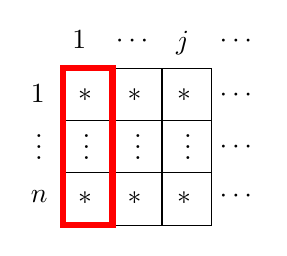
\begin{tikzpicture}[x=0.75pt,y=0.75pt,yscale=-1,xscale=1]
%uncomment if require: \path (0,534); %set diagram left start at 0, and has height of 534

%Shape: Rectangle [id:dp17271303952502315] 
% \draw   (52.81,325.2) -- (76.62,325.2) -- (76.62,350.41) -- (52.81,350.41) -- cycle ;
%Shape: Rectangle [id:dp4366577772656428] 
\draw   (76.81,350.41) -- (100.62,350.41) -- (100.62,375.62) -- (76.81,375.62) -- cycle ;
%Shape: Rectangle [id:dp13823281826780653] 
\draw   (76.81,325.2) -- (100.62,325.2) -- (100.62,350.41) -- (76.81,350.41) -- cycle ;
%Shape: Rectangle [id:dp25508926192152326] 
\draw   (100.62,325.2) -- (124.43,325.2) -- (124.43,350.41) -- (100.62,350.41) -- cycle ;
%Shape: Rectangle [id:dp7615695748694848] 
\draw   (124.43,325.2) -- (148.24,325.2) -- (148.24,350.41) -- (124.43,350.41) -- cycle ;
%Shape: Rectangle [id:dp7082057113045306] 
\draw   (100.62,350.41) -- (124.43,350.41) -- (124.43,375.62) -- (100.62,375.62) -- cycle ;
%Shape: Rectangle [id:dp5459336420864682] 
\draw   (124.43,350.41) -- (148.24,350.41) -- (148.24,375.62) -- (124.43,375.62) -- cycle ;
%Shape: Rectangle [id:dp8229762223203931] 
\draw   (76.81,375.62) -- (100.62,375.62) -- (100.62,400.83) -- (76.81,400.83) -- cycle ;
%Shape: Rectangle [id:dp7425833826219033] 
\draw   (100.62,375.62) -- (124.43,375.62) -- (124.43,400.83) -- (100.62,400.83) -- cycle ;
%Shape: Rectangle [id:dp11427372040336436] 
\draw   (124.43,375.62) -- (148.24,375.62) -- (148.24,400.83) -- (124.43,400.83) -- cycle ;
%Shape: Rectangle [id:dp835448558688529] 
\draw  [color={rgb, 255:red, 255; green, 0; blue, 0 }  ,draw opacity=1 ][line width=2.25]  (76.81,325.2) -- (100.62,325.2) -- (100.62,400.83) -- (76.81,400.83) -- cycle ;

% Text Node
\draw (82.82,334.01) node [anchor=north west][inner sep=0.75pt]    {$*$};
% Text Node
\draw (106.63,334.01) node [anchor=north west][inner sep=0.75pt]    {$*$};
% Text Node
\draw (130.44,334.01) node [anchor=north west][inner sep=0.75pt]    {$*$};
% Text Node
\draw (82.82,383.43) node [anchor=north west][inner sep=0.75pt]    {$*$};
% Text Node
\draw (106.63,383.43) node [anchor=north west][inner sep=0.75pt]    {$*$};
% Text Node
\draw (130.44,383.43) node [anchor=north west][inner sep=0.75pt]    {$*$};
% Text Node
\draw (62,348) node [anchor=north west][inner sep=0.75pt]    {$\vdots $};
% Text Node
\draw (60,332) node [anchor=north west][inner sep=0.75pt]    {$1$};
% Text Node
\draw (60,383) node [anchor=north west][inner sep=0.75pt]    {$n$};
% Text Node
\draw (85,348) node [anchor=north west][inner sep=0.75pt]    {$\vdots $};
% Text Node
\draw (109.81,348) node [anchor=north west][inner sep=0.75pt]    {$\vdots $};
% Text Node
\draw (133.81,348) node [anchor=north west][inner sep=0.75pt]    {$\vdots $};
% Text Node
\draw (80,306) node [anchor=north west][inner sep=0.75pt]    {$1$};
% Text Node
\draw (101,308) node [anchor=north west][inner sep=0.75pt]    {$\cdots $};
% Text Node
\draw (130,306) node [anchor=north west][inner sep=0.75pt]    {$j$};
% Text Node
\draw (151,308) node [anchor=north west][inner sep=0.75pt]    {$\cdots $};
% Text Node
\draw (151,334) node [anchor=north west][inner sep=0.75pt]    {$\cdots $};
% Text Node
\draw (151,359) node [anchor=north west][inner sep=0.75pt]    {$\cdots $};
% Text Node
\draw (151,383) node [anchor=north west][inner sep=0.75pt]    {$\cdots $};
% Text Node
% \draw (57.82,334.01) node [anchor=north west][inner sep=0.75pt]    {$*$};


\end{tikzpicture}
\vspace{0.15em}\pause
\end{column}\pause
\begin{column}{.1\textwidth}
\centering $\overset{\text{resampling $X_1$}}{\follows}$
\end{column}
\begin{column}{.3\textwidth}



\tikzset{every picture/.style={line width=0.75pt}} %set default line width to 0.75pt        

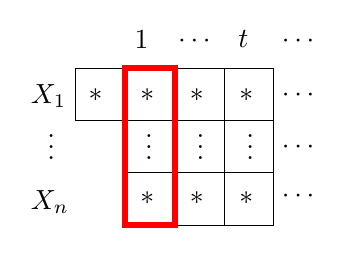
\begin{tikzpicture}[x=0.75pt,y=0.75pt,yscale=-1,xscale=1]
%uncomment if require: \path (0,534); %set diagram left start at 0, and has height of 534

%Shape: Rectangle [id:dp17271303952502315] 
\draw   (52.81,325.2) -- (76.62,325.2) -- (76.62,350.41) -- (52.81,350.41) -- cycle ;
%Shape: Rectangle [id:dp4366577772656428] 
\draw   (76.81,350.41) -- (100.62,350.41) -- (100.62,375.62) -- (76.81,375.62) -- cycle ;
%Shape: Rectangle [id:dp13823281826780653] 
\draw   (76.81,325.2) -- (100.62,325.2) -- (100.62,350.41) -- (76.81,350.41) -- cycle ;
%Shape: Rectangle [id:dp25508926192152326] 
\draw   (100.62,325.2) -- (124.43,325.2) -- (124.43,350.41) -- (100.62,350.41) -- cycle ;
%Shape: Rectangle [id:dp7615695748694848] 
\draw   (124.43,325.2) -- (148.24,325.2) -- (148.24,350.41) -- (124.43,350.41) -- cycle ;
%Shape: Rectangle [id:dp7082057113045306] 
\draw   (100.62,350.41) -- (124.43,350.41) -- (124.43,375.62) -- (100.62,375.62) -- cycle ;
%Shape: Rectangle [id:dp5459336420864682] 
\draw   (124.43,350.41) -- (148.24,350.41) -- (148.24,375.62) -- (124.43,375.62) -- cycle ;
%Shape: Rectangle [id:dp8229762223203931] 
\draw   (76.81,375.62) -- (100.62,375.62) -- (100.62,400.83) -- (76.81,400.83) -- cycle ;
%Shape: Rectangle [id:dp7425833826219033] 
\draw   (100.62,375.62) -- (124.43,375.62) -- (124.43,400.83) -- (100.62,400.83) -- cycle ;
%Shape: Rectangle [id:dp11427372040336436] 
\draw   (124.43,375.62) -- (148.24,375.62) -- (148.24,400.83) -- (124.43,400.83) -- cycle ;
%Shape: Rectangle [id:dp835448558688529] 
\draw  [color={rgb, 255:red, 255; green, 0; blue, 0 }  ,draw opacity=1 ][line width=2.25]  (76.81,325.2) -- (100.62,325.2) -- (100.62,400.83) -- (76.81,400.83) -- cycle ;

% Text Node
\draw (82.82,334.01) node [anchor=north west][inner sep=0.75pt]    {$*$};
% Text Node
\draw (106.63,334.01) node [anchor=north west][inner sep=0.75pt]    {$*$};
% Text Node
\draw (130.44,334.01) node [anchor=north west][inner sep=0.75pt]    {$*$};
% Text Node
\draw (82.82,383.43) node [anchor=north west][inner sep=0.75pt]    {$*$};
% Text Node
\draw (106.63,383.43) node [anchor=north west][inner sep=0.75pt]    {$*$};
% Text Node
\draw (130.44,383.43) node [anchor=north west][inner sep=0.75pt]    {$*$};
% Text Node
\draw (38,348) node [anchor=north west][inner sep=0.75pt]    {$\vdots $};
% Text Node
\draw (30,332) node [anchor=north west][inner sep=0.75pt]    {$X_1$};
% Text Node
\draw (30,383) node [anchor=north west][inner sep=0.75pt]    {$X_n$};
% Text Node
\draw (85,348) node [anchor=north west][inner sep=0.75pt]    {$\vdots $};
% Text Node
\draw (109.81,348) node [anchor=north west][inner sep=0.75pt]    {$\vdots $};
% Text Node
\draw (133.81,348) node [anchor=north west][inner sep=0.75pt]    {$\vdots $};
% Text Node
\draw (80,306) node [anchor=north west][inner sep=0.75pt]    {$1$};
% Text Node
\draw (101,308) node [anchor=north west][inner sep=0.75pt]    {$\cdots $};
% Text Node
\draw (130,306) node [anchor=north west][inner sep=0.75pt]    {$t$};
% Text Node
\draw (151,308) node [anchor=north west][inner sep=0.75pt]    {$\cdots $};
% Text Node
\draw (151,334) node [anchor=north west][inner sep=0.75pt]    {$\cdots $};
% Text Node
\draw (151,359) node [anchor=north west][inner sep=0.75pt]    {$\cdots $};
% Text Node
\draw (151,383) node [anchor=north west][inner sep=0.75pt]    {$\cdots $};
% Text Node
\draw (57.82,334.01) node [anchor=north west][inner sep=0.75pt]    {$*$};


\end{tikzpicture}

\end{column}
\begin{column}{.05\textwidth}
\end{column}
\end{columns}\pause

When resampling $B_i$, shift rows $\var{B_i}$ to left.\pause\padding

\follows MT algorithm deterministic with respect to resampling table!
\end{frame}

% \subsection{Outline}
% \begin{frame}{Outline}
%     Goal: Find a resampling table such that after poly. resamples all bad-events are avoided.\spadding
    
%     Idea: Choose $R$ such that the MT algorithm only performs resamples that the randomized variant is likely to perform.\pause\padding
    
%     \begin{enumerate}
%         \item Construct set of unlikely resamples of randomized MT algorithm.\pause
%         \item Use method of conditional expectations to find a resampling table $R$ such that all of these resamplings are avoided.\pause
%         \item Simulate MT algorithm using $R$.
%     \end{enumerate}
% \end{frame}

\subsection{Counting Resamples}
\begin{frame}{Counting Resamples}
% Find an injective mapping from resamples to some ``countable'' structure.\pause
Want to find an encoding of resamples such that we do not lose much information.\pause

\begin{block}{Why may executions be long?}
Given a resampling table $R$, a \b{(partial) execution} of the MT algorithm is described by the sequence of resampled bad-events.\pause\spadding

\begin{columns}
\begin{column}{.15\textwidth}
\centering $B_1, B_2, B_3\onslide<5->{, \r{B_4}}$
\end{column}
\begin{column}{.0\textwidth}
\centering $\mapsto$
\end{column}\pause
\begin{column}{.2\textwidth}
\centering


\tikzset{every picture/.style={line width=0.75pt}} %set default line width to 0.75pt        

\hspace{-1.3em}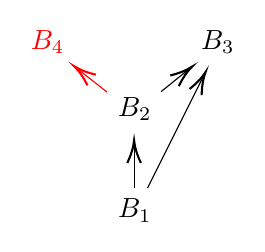
\begin{tikzpicture}[x=0.75pt,y=0.75pt,yscale=-1,xscale=1]
%uncomment if require: \path (0,534); %set diagram left start at 0, and has height of 534


% Text Node
\onslide<5->{\draw (241,27) node [anchor=north west][inner sep=0.75pt]  [color={rgb, 255:red, 255; green, 0; blue, 0 }  ,opacity=1 ]    {$B_{4}$};}
% Text Node
\draw (283,59) node [anchor=north west][inner sep=0.75pt]    {$B_{2}$};
% Text Node
\draw (323,27) node [anchor=north west][inner sep=0.75pt]    {$B_{3}$};
% Text Node
\draw (283,108) node [anchor=north west][inner sep=0.75pt]    {$B_{1}$};
% Connection
\onslide<5->{\draw [color={rgb, 255:red, 255; green, 0; blue, 0 }  ,draw opacity=1 ]    (279,57.79) -- (264.57,46.45) ;
\draw [shift={(263,45.21)}, rotate = 38.16] [color={rgb, 255:red, 255; green, 0; blue, 0 }  ][line width=0.75]    (10.93,-3.29) .. controls (6.95,-1.4) and (3.31,-0.3) .. (0,0) .. controls (3.31,0.3) and (6.95,1.4) .. (10.93,3.29)   ;}
% Connection
\draw    (305,57.54) -- (318.44,46.72) ;
\draw [shift={(320,45.46)}, rotate = 141.17] [color={rgb, 255:red, 0; green, 0; blue, 0 }  ][line width=0.75]    (10.93,-3.29) .. controls (6.95,-1.4) and (3.31,-0.3) .. (0,0) .. controls (3.31,0.3) and (6.95,1.4) .. (10.93,3.29)   ;
% Connection
\draw    (292,83) -- (292,104) ;
\draw [shift={(292,81)}, rotate = 90] [color={rgb, 255:red, 0; green, 0; blue, 0 }  ][line width=0.75]    (10.93,-3.29) .. controls (6.95,-1.4) and (3.31,-0.3) .. (0,0) .. controls (3.31,0.3) and (6.95,1.4) .. (10.93,3.29)   ;
% Connection
\draw    (298.5,104) -- (325.61,49.79) ;
\draw [shift={(326.5,48)}, rotate = 116.57] [color={rgb, 255:red, 0; green, 0; blue, 0 }  ][line width=0.75]    (10.93,-3.29) .. controls (6.95,-1.4) and (3.31,-0.3) .. (0,0) .. controls (3.31,0.3) and (6.95,1.4) .. (10.93,3.29)   ;

\end{tikzpicture}

\end{column}
\begin{column}{.3\textwidth}
\b{Witness DAG} $\hat{G}$

$B_i \longrightarrow B_j$ iff $i < j$\par and $B_i$ affects $B_j$
\end{column}
\end{columns}\pause\pause

\follows $\hat{G}$ is always a DAG!\pause\ But why are DAGs a good encoding?
\end{block}
\end{frame}

\begin{frame}{Counting Resamples}
Witness DAGs encode the final configuration of the MT algorithm!\spadding

\begin{columns}[T]
\begin{column}{.4\textwidth}
\centering\vspace{-1em}


\tikzset{every picture/.style={line width=0.75pt}} %set default line width to 0.75pt        

\begin{tikzpicture}[x=0.75pt,y=0.75pt,yscale=-1,xscale=1]
%uncomment if require: \path (0,534); %set diagram left start at 0, and has height of 534


% Text Node
\only<1-5,7-8>{\draw (241,27) node [anchor=north west][inner sep=0.75pt]    {$B_{4}$};}
\only<6,9->{\draw (241,27) node [anchor=north west][inner sep=0.75pt]  [color={rgb, 255:red, 255; green, 0; blue, 0 }  ,opacity=1 ]    {$B_{4}$};}
% Text Node
\only<1-3>{\draw (283,59) node [anchor=north west][inner sep=0.75pt]    {$B_{2}$};}
\only<4->{\draw (283,59) node [anchor=north west][inner sep=0.75pt]  [color={rgb, 255:red, 124; green, 216; blue, 23 }  ,opacity=1 ]    {$B_{2}$};}
% Text Node
\only<1-4,8-9>{\draw (323,27) node [anchor=north west][inner sep=0.75pt]    {$B_{3}$};}
\only<5-7,10->{\draw (323,27) node [anchor=north west][inner sep=0.75pt]  [color={rgb, 255:red, 250; green, 153; blue, 3 }  ,opacity=1 ]    {$B_{3}$};}
% Text Node
\only<1-2>{\draw (283,108) node [anchor=north west][inner sep=0.75pt]    {$B_{1}$};}
\only<3->{\draw (283,108) node [anchor=north west][inner sep=0.75pt]  [color={rgb, 255:red, 0; green, 0; blue, 255 }  ,opacity=1 ]    {$B_{1}$};}
% Connection
\draw    (279,57.79) -- (264.57,46.45) ;
\draw [shift={(263,45.21)}, rotate = 38.16] [color={rgb, 255:red, 0; green, 0; blue, 0 }  ][line width=0.75]    (10.93,-3.29) .. controls (6.95,-1.4) and (3.31,-0.3) .. (0,0) .. controls (3.31,0.3) and (6.95,1.4) .. (10.93,3.29)   ;
% Connection
\draw    (305,57.54) -- (318.44,46.72) ;
\draw [shift={(320,45.46)}, rotate = 141.17] [color={rgb, 255:red, 0; green, 0; blue, 0 }  ][line width=0.75]    (10.93,-3.29) .. controls (6.95,-1.4) and (3.31,-0.3) .. (0,0) .. controls (3.31,0.3) and (6.95,1.4) .. (10.93,3.29)   ;
% Connection
\draw    (292,83) -- (292,104) ;
\draw [shift={(292,81)}, rotate = 90] [color={rgb, 255:red, 0; green, 0; blue, 0 }  ][line width=0.75]    (10.93,-3.29) .. controls (6.95,-1.4) and (3.31,-0.3) .. (0,0) .. controls (3.31,0.3) and (6.95,1.4) .. (10.93,3.29)   ;
% Connection
\draw    (298.5,104) -- (325.61,49.79) ;
\draw [shift={(326.5,48)}, rotate = 116.57] [color={rgb, 255:red, 0; green, 0; blue, 0 }  ][line width=0.75]    (10.93,-3.29) .. controls (6.95,-1.4) and (3.31,-0.3) .. (0,0) .. controls (3.31,0.3) and (6.95,1.4) .. (10.93,3.29)   ;

\onslide<15->{\draw (228,73) node [anchor=north west][inner sep=0.75pt]  [color={rgb, 255:red, 255; green, 0; blue, 0 }  ,opacity=1 ]  {$\hat{G}(B_{4})$};

%Curve Lines [id:da02533473137358766] 
\draw [color={rgb, 255:red, 255; green, 0; blue, 0 }  ,draw opacity=1 ]   (260,24) .. controls (299,48) and (316,61) .. (309,110) ;
%Curve Lines [id:da2150259195395825] 
\draw [color={rgb, 255:red, 255; green, 0; blue, 0 }  ,draw opacity=1 ]   (244,48) .. controls (225,35) and (242,13) .. (260,24) ;
%Curve Lines [id:da46500745717824676] 
\draw [color={rgb, 255:red, 255; green, 0; blue, 0 }  ,draw opacity=1 ]   (244,48) .. controls (284,73) and (282,73) .. (279,107) ;
%Curve Lines [id:da9402495253404746] 
\draw [color={rgb, 255:red, 255; green, 0; blue, 0 }  ,draw opacity=1 ]   (309,110) .. controls (308,134) and (276,145) .. (279,107) ;}

\end{tikzpicture}
\vspace{-1.5em}\spadding

{\small
\vspace{-2em}\begin{align*}
\var{B_1} = \{X_1,X_3,X_5\} \\
\var{B_2} = \{X_2,X_3,X_6\} \\
\var{B_3} = \{X_1,X_5,X_6\} \\
\var{B_4} = \{X_2,X_4,X_7\}
\end{align*}
}
\end{column}\pause
\begin{column}{.4\textwidth}
\centering


\tikzset{every picture/.style={line width=0.75pt}} %set default line width to 0.75pt        

\begin{tikzpicture}[x=0.75pt,y=0.75pt,yscale=-1,xscale=1,scale=0.75]
%uncomment if require: \path (0,534); %set diagram left start at 0, and has height of 534

%Shape: Rectangle [id:dp13823281826780653] 
\draw   (76.81,325.2) -- (100.62,325.2) -- (100.62,350.41) -- (76.81,350.41) -- cycle ;
%Shape: Rectangle [id:dp25508926192152326] 
\draw   (100.62,325.2) -- (124.43,325.2) -- (124.43,350.41) -- (100.62,350.41) -- cycle ;
%Shape: Rectangle [id:dp7615695748694848] 
\draw   (124.43,325.2) -- (148.24,325.2) -- (148.24,350.41) -- (124.43,350.41) -- cycle ;
%Shape: Rectangle [id:dp4366577772656428] 
\draw   (76.81,350.41) -- (100.62,350.41) -- (100.62,375.62) -- (76.81,375.62) -- cycle ;
%Shape: Rectangle [id:dp7082057113045306] 
\draw   (100.62,350.41) -- (124.43,350.41) -- (124.43,375.62) -- (100.62,375.62) -- cycle ;
%Shape: Rectangle [id:dp5459336420864682] 
\draw   (124.43,350.41) -- (148.24,350.41) -- (148.24,375.62) -- (124.43,375.62) -- cycle ;
%Shape: Rectangle [id:dp8229762223203931] 
\draw   (76.81,375.62) -- (100.62,375.62) -- (100.62,400.83) -- (76.81,400.83) -- cycle ;
%Shape: Rectangle [id:dp7425833826219033] 
\draw   (100.62,375.62) -- (124.43,375.62) -- (124.43,400.83) -- (100.62,400.83) -- cycle ;
%Shape: Rectangle [id:dp11427372040336436] 
\draw   (124.43,375.62) -- (148.24,375.62) -- (148.24,400.83) -- (124.43,400.83) -- cycle ;
%Shape: Rectangle [id:dp8229762223203931] 
\draw   (76.81,400.62) -- (100.62,400.62) -- (100.62,425.83) -- (76.81,425.83) -- cycle ;
%Shape: Rectangle [id:dp7425833826219033] 
\draw   (100.62,400.62) -- (124.43,400.62) -- (124.43,425.83) -- (100.62,425.83) -- cycle ;
%Shape: Rectangle [id:dp11427372040336436] 
\draw   (124.43,400.62) -- (148.24,400.62) -- (148.24,425.83) -- (124.43,425.83) -- cycle ;
%Shape: Rectangle [id:dp8229762223203931] 
\draw   (76.81,425.62) -- (100.62,425.62) -- (100.62,450.83) -- (76.81,450.83) -- cycle ;
%Shape: Rectangle [id:dp7425833826219033] 
\draw   (100.62,425.62) -- (124.43,425.62) -- (124.43,450.83) -- (100.62,450.83) -- cycle ;
%Shape: Rectangle [id:dp11427372040336436] 
\draw   (124.43,425.62) -- (148.24,425.62) -- (148.24,450.83) -- (124.43,450.83) -- cycle ;
%Shape: Rectangle [id:dp8229762223203931] 
\draw   (76.81,450.62) -- (100.62,450.62) -- (100.62,475.83) -- (76.81,475.83) -- cycle ;
%Shape: Rectangle [id:dp7425833826219033] 
\draw   (100.62,450.62) -- (124.43,450.62) -- (124.43,475.83) -- (100.62,475.83) -- cycle ;
%Shape: Rectangle [id:dp11427372040336436] 
\draw   (124.43,450.62) -- (148.24,450.62) -- (148.24,475.83) -- (124.43,475.83) -- cycle ;
%Shape: Rectangle [id:dp8229762223203931] 
\draw   (76.81,475.62) -- (100.62,475.62) -- (100.62,500.83) -- (76.81,500.83) -- cycle ;
%Shape: Rectangle [id:dp7425833826219033] 
\draw   (100.62,475.62) -- (124.43,475.62) -- (124.43,500.83) -- (100.62,500.83) -- cycle ;
%Shape: Rectangle [id:dp11427372040336436] 
\draw   (124.43,475.62) -- (148.24,475.62) -- (148.24,500.83) -- (124.43,500.83) -- cycle ;

% Text Node
\draw (81.82,332.01) node [anchor=north west][inner sep=0.75pt]    {$*$};
% Text Node
\draw (105.63,332.01) node [anchor=north west][inner sep=0.75pt]    {$*$};
% Text Node
\draw (129.44,332.01) node [anchor=north west][inner sep=0.75pt]    {$*$};
% Text Node
\draw (81.82,357.01) node [anchor=north west][inner sep=0.75pt]    {$*$};
% Text Node
\draw (105.63,357.01) node [anchor=north west][inner sep=0.75pt]    {$*$};
% Text Node
\draw (129.44,357.01) node [anchor=north west][inner sep=0.75pt]    {$*$};
% Text Node
\draw (81.82,382.01) node [anchor=north west][inner sep=0.75pt]    {$*$};
% Text Node
\draw (105.63,382.01) node [anchor=north west][inner sep=0.75pt]    {$*$};
% Text Node
\draw (129.44,382.01) node [anchor=north west][inner sep=0.75pt]    {$*$};
% Text Node
\draw (81.82,407.01) node [anchor=north west][inner sep=0.75pt]    {$*$};
% Text Node
\draw (105.63,407.01) node [anchor=north west][inner sep=0.75pt]    {$*$};
% Text Node
\draw (129.44,407.01) node [anchor=north west][inner sep=0.75pt]    {$*$};
% Text Node
\draw (81.82,432.01) node [anchor=north west][inner sep=0.75pt]    {$*$};
% Text Node
\draw (105.63,432.01) node [anchor=north west][inner sep=0.75pt]    {$*$};
% Text Node
\draw (129.44,432.01) node [anchor=north west][inner sep=0.75pt]    {$*$};
% Text Node
\draw (81.82,457.01) node [anchor=north west][inner sep=0.75pt]    {$*$};
% Text Node
\draw (105.63,457.01) node [anchor=north west][inner sep=0.75pt]    {$*$};
% Text Node
\draw (129.44,457.01) node [anchor=north west][inner sep=0.75pt]    {$*$};
% Text Node
\draw (81.82,482.01) node [anchor=north west][inner sep=0.75pt]    {$*$};
% Text Node
\draw (105.63,482.01) node [anchor=north west][inner sep=0.75pt]    {$*$};
% Text Node
\draw (129.44,482.01) node [anchor=north west][inner sep=0.75pt]    {$*$};
% Text Node
\draw (185,329) node [anchor=north west][inner sep=0.75pt]  [opacity=0.5]    {\small$X_1$};
% Text Node
\draw (185,354) node [anchor=north west][inner sep=0.75pt]  [opacity=0.5]    {\small$X_2$};
% Text Node
\draw (185,379) node [anchor=north west][inner sep=0.75pt]  [opacity=0.5]    {\small$X_3$};
% Text Node
\draw (185,404) node [anchor=north west][inner sep=0.75pt]  [opacity=0.5]    {\small$X_4$};
% Text Node
\draw (185,429) node [anchor=north west][inner sep=0.75pt]  [opacity=0.5]    {\small$X_5$};
% Text Node
\draw (185,454) node [anchor=north west][inner sep=0.75pt]  [opacity=0.5]    {\small$X_6$};
% Text Node
\draw (185,479) node [anchor=north west][inner sep=0.75pt]  [opacity=0.5]    {\small$X_7$};
% Text Node
\draw (151,332) node [anchor=north west][inner sep=0.75pt]    {$\cdots $};
% Text Node
\draw (151,357) node [anchor=north west][inner sep=0.75pt]    {$\cdots $};
% Text Node
\draw (151,382) node [anchor=north west][inner sep=0.75pt]    {$\cdots $};
% Text Node
\draw (151,407) node [anchor=north west][inner sep=0.75pt]    {$\cdots $};
% Text Node
\draw (151,432) node [anchor=north west][inner sep=0.75pt]    {$\cdots $};
% Text Node
\draw (151,457) node [anchor=north west][inner sep=0.75pt]    {$\cdots $};
% Text Node
\draw (151,482) node [anchor=north west][inner sep=0.75pt]    {$\cdots $};


\only<3->{\draw (56.82,332.01) node [anchor=north west][inner sep=0.75pt]    {$*$};}
\only<3->{\draw (56.82,382.01) node [anchor=north west][inner sep=0.75pt]    {$*$};}
\only<3->{\draw (56.82,432.01) node [anchor=north west][inner sep=0.75pt]    {$*$};}
\only<4->{\draw (56.82,357.01) node [anchor=north west][inner sep=0.75pt]    {$*$};}
\only<4->{\draw (31.82,382.01) node [anchor=north west][inner sep=0.75pt]    {$*$};}
\only<4->{\draw (56.82,457.01) node [anchor=north west][inner sep=0.75pt]    {$*$};}
\only<5-7,10->{\draw (31.82,332.01) node [anchor=north west][inner sep=0.75pt]    {$*$};}
\only<5-7,10->{\draw (31.82,432.01) node [anchor=north west][inner sep=0.75pt]    {$*$};}
\only<5-7,10->{\draw (31.82,457.01) node [anchor=north west][inner sep=0.75pt]    {$*$};}
\only<6,9->{\draw (31.82,357.01) node [anchor=north west][inner sep=0.75pt]    {$*$};}
\only<6,9->{\draw (56.82,407.01) node [anchor=north west][inner sep=0.75pt]    {$*$};}
\only<6,9->{\draw (56.82,482.01) node [anchor=north west][inner sep=0.75pt]    {$*$};}

\only<3-4,8-9>{\draw  [fill={rgb, 255:red, 0; green, 0; blue, 255 }  ,fill opacity=0.3 ]   (51.81,325.2) -- (75.62,325.2) -- (75.62,350.41) -- (51.81,350.41) -- cycle ;}
\only<5-7,10->{\draw  [fill={rgb, 255:red, 0; green, 0; blue, 255 }  ,fill opacity=0.3 ]   (27.81,325.2) -- (51.62,325.2) -- (51.62,350.41) -- (27.81,350.41) -- cycle ;}
\only<5-7,10->{\draw  [fill={rgb, 255:red, 250; green, 153; blue, 3 }  ,fill opacity=0.3 ]   (51.81,325.2) -- (75.62,325.2) -- (75.62,350.41) -- (51.81,350.41) -- cycle ;}

\only<4-5,7-8>{\draw  [fill={rgb, 255:red, 0; green, 255; blue, 0 }  ,fill opacity=0.3 ]   (51.81,350.2) -- (75.62,350.2) -- (75.62,375.41) -- (51.81,375.41) -- cycle ;}
\only<6,9->{\draw  [fill={rgb, 255:red, 0; green, 255; blue, 0 }  ,fill opacity=0.3 ]   (27.81,350.2) -- (51.62,350.2) -- (51.62,375.41) -- (27.81,375.41) -- cycle ;}
\only<6,9->{\draw  [fill={rgb, 255:red, 255; green, 0; blue, 0 }  ,fill opacity=0.3 ]   (51.81,350.2) -- (75.62,350.2) -- (75.62,375.41) -- (51.81,375.41) -- cycle ;}

\only<3>{\draw  [fill={rgb, 255:red, 0; green, 0; blue, 255 }  ,fill opacity=0.3 ]   (51.81,375.2) -- (75.62,375.2) -- (75.62,400.41) -- (51.81,400.41) -- cycle ;}
\onslide<4->{\draw  [fill={rgb, 255:red, 0; green, 0; blue, 255 }  ,fill opacity=0.3 ]   (27.81,375.2) -- (51.62,375.2) -- (51.62,400.41) -- (27.81,400.41) -- cycle ;}
\onslide<4->{\draw  [fill={rgb, 255:red, 0; green, 255; blue, 0 }  ,fill opacity=0.3 ]   (51.81,375.2) -- (75.62,375.2) -- (75.62,400.41) -- (51.81,400.41) -- cycle ;}

\only<6,9->{\draw  [fill={rgb, 255:red, 255; green, 0; blue, 0 }  ,fill opacity=0.3 ]   (51.81,400.2) -- (75.62,400.2) -- (75.62,425.41) -- (51.81,425.41) -- cycle ;}

\only<3-4,8-9>{\draw  [fill={rgb, 255:red, 0; green, 0; blue, 255 }  ,fill opacity=0.3 ]   (51.81,425.2) -- (75.62,425.2) -- (75.62,450.41) -- (51.81,450.41) -- cycle ;}
\only<5-7,10->{\draw  [fill={rgb, 255:red, 0; green, 0; blue, 255 }  ,fill opacity=0.3 ]   (27.81,425.2) -- (51.62,425.2) -- (51.62,450.41) -- (27.81,450.41) -- cycle ;}
\only<5-7,10->{\draw  [fill={rgb, 255:red, 250; green, 153; blue, 3 }  ,fill opacity=0.3 ]   (51.81,425.2) -- (75.62,425.2) -- (75.62,450.41) -- (51.81,450.41) -- cycle ;}

\only<4,8-9>{\draw  [fill={rgb, 255:red, 0; green, 255; blue, 0 }  ,fill opacity=0.3 ]   (51.81,450.2) -- (75.62,450.2) -- (75.62,475.41) -- (51.81,475.41) -- cycle ;}
\only<5-7,10->{\draw  [fill={rgb, 255:red, 0; green, 255; blue, 0 }  ,fill opacity=0.3 ]   (27.81,450.2) -- (51.62,450.2) -- (51.62,475.41) -- (27.81,475.41) -- cycle ;}
\only<5-7,10->{\draw  [fill={rgb, 255:red, 250; green, 153; blue, 3 }  ,fill opacity=0.3 ]   (51.81,450.2) -- (75.62,450.2) -- (75.62,475.41) -- (51.81,475.41) -- cycle ;}

\only<6,9->{\draw  [fill={rgb, 255:red, 255; green, 0; blue, 0 }  ,fill opacity=0.3 ]   (51.81,475.2) -- (75.62,475.2) -- (75.62,500.41) -- (51.81,500.41) -- cycle ;}


%Shape: Rectangle [id:dp835448558688529] 
\onslide<2-13>{\draw  [color={rgb, 255:red, 255; green, 0; blue, 0 }  ,draw opacity=1 ][line width=2.25]  (76.81,325.2) -- (100.62,325.2) -- (100.62,500.83) -- (76.81,500.83) -- cycle ;}
\onslide<14->{\draw  [color={rgb, 255:red, 255; green, 0; blue, 0 }  ,draw opacity=1 ][line width=2.25]  (76.81,350.2) -- (100.62,350.2) -- (100.62,375.83) -- (76.81,375.83) -- cycle ;
\draw  [color={rgb, 255:red, 255; green, 0; blue, 0 }  ,draw opacity=1 ][line width=2.25]  (76.81,400.2) -- (100.62,400.2) -- (100.62,425.83) -- (76.81,425.83) -- cycle ;
\draw  [color={rgb, 255:red, 255; green, 0; blue, 0 }  ,draw opacity=1 ][line width=2.25]  (76.81,475.2) -- (100.62,475.2) -- (100.62,500.83) -- (76.81,500.83) -- cycle ;}


\end{tikzpicture}
\spadding

\onslide<2->{fixed resampling table $R$}
\onslide<3->{resamples: \b{$B_1$}}\onslide<4->{, \textcolor{softgreen}{$B_2$}}\only<5-7>{, \textcolor{orange}{$B_3$}}\onslide<6,9->{, \r{$B_4$}}\onslide<10->{, \textcolor{orange}{$B_3$}}
\end{column}
\begin{column}{.1\textwidth}
\end{column}
\end{columns}\spadding

\onslide<11->{\follows may encode multiple executions, but \emph{all} lead to the same final configuration!}

\onslide<12->{\follows resampled bad-events depend on \emph{disjoint} entries of $R$!}

\onslide<13->{\follows configuration at step $t$ is drawn according to $\distr$!}
\end{frame}

% \begin{frame}{Counting Resamples}
% \begin{block}{Witness DAG of resamples}
% \begin{center}
% 


\tikzset{every picture/.style={line width=0.75pt}} %set default line width to 0.75pt        

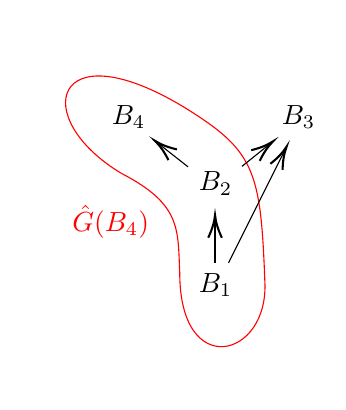
\begin{tikzpicture}[x=0.75pt,y=0.75pt,yscale=-1,xscale=1]
%uncomment if require: \path (0,534); %set diagram left start at 0, and has height of 534

\draw (222,75) node [anchor=north west][inner sep=0.75pt]  [color={rgb, 255:red, 255; green, 0; blue, 0 }  ,opacity=1 ]  {$\hat{G}(B_{4})$};

%Curve Lines [id:da8086917494340398] 
\draw [color={rgb, 255:red, 255; green, 0; blue, 0 }  ,draw opacity=1 ]   (277,29) .. controls (311,50) and (314,59) .. (316,113) ;
%Curve Lines [id:da21472780558540894] 
\draw [color={rgb, 255:red, 255; green, 0; blue, 0 }  ,draw opacity=1 ]   (247,61) .. controls (202,34) and (214,-9) .. (277,29) ;
%Curve Lines [id:da2557925845138229] 
\draw [color={rgb, 255:red, 255; green, 0; blue, 0 }  ,draw opacity=1 ]   (247,61) .. controls (276,76) and (274,88) .. (275,109) ;
%Curve Lines [id:da06777553579467122] 
\draw [color={rgb, 255:red, 255; green, 0; blue, 0 }  ,draw opacity=1 ]   (316,113) .. controls (318,150) and (275,161) .. (275,109) ;


% Text Node
\draw (241,27) node [anchor=north west][inner sep=0.75pt]    {$B_{4}$};
% Text Node
\draw (283,59) node [anchor=north west][inner sep=0.75pt]    {$B_{2}$};
% Text Node
\draw (323,27) node [anchor=north west][inner sep=0.75pt]    {$B_{3}$};
% Text Node
\draw (283,108) node [anchor=north west][inner sep=0.75pt]    {$B_{1}$};
% Connection
\draw    (279,57.79) -- (264.57,46.45) ;
\draw [shift={(263,45.21)}, rotate = 38.16] [color={rgb, 255:red, 0; green, 0; blue, 0 }  ][line width=0.75]    (10.93,-3.29) .. controls (6.95,-1.4) and (3.31,-0.3) .. (0,0) .. controls (3.31,0.3) and (6.95,1.4) .. (10.93,3.29)   ;
% Connection
\draw    (305,57.54) -- (318.44,46.72) ;
\draw [shift={(320,45.46)}, rotate = 141.17] [color={rgb, 255:red, 0; green, 0; blue, 0 }  ][line width=0.75]    (10.93,-3.29) .. controls (6.95,-1.4) and (3.31,-0.3) .. (0,0) .. controls (3.31,0.3) and (6.95,1.4) .. (10.93,3.29)   ;
% Connection
\draw    (292,83) -- (292,104) ;
\draw [shift={(292,81)}, rotate = 90] [color={rgb, 255:red, 0; green, 0; blue, 0 }  ][line width=0.75]    (10.93,-3.29) .. controls (6.95,-1.4) and (3.31,-0.3) .. (0,0) .. controls (3.31,0.3) and (6.95,1.4) .. (10.93,3.29)   ;
% Connection
\draw    (298.5,104) -- (325.61,49.79) ;
\draw [shift={(326.5,48)}, rotate = 116.57] [color={rgb, 255:red, 0; green, 0; blue, 0 }  ][line width=0.75]    (10.93,-3.29) .. controls (6.95,-1.4) and (3.31,-0.3) .. (0,0) .. controls (3.31,0.3) and (6.95,1.4) .. (10.93,3.29)   ;

\end{tikzpicture}

% \end{center}

% Observe: Given a resampling table $R$, $\hat{G}(B_t)$ explains the values of $\var{B_t}$ before \& after resampling $B_t$.\pause\spadding

% \follows we have an injective mapping!
% \end{block}
% \end{frame}

\subsection{Analyzing the MT Algorithm}
\begin{frame}{Analyzing the MT Algorithm}
Are \emph{all} witness DAGs used as an encoding of a resample?\pause\par
No! \follows we can improve our counting!\pause\spadding

\begin{itemize}
    \item $\hat{G}(B_i)$ always has a single sink (set denoted $\G$)\pause
    \item If we fix a resampling table $R$, do we need to consider all single-sink witness DAGs $G$?\pause
    
    \follows No! \pause$G$ \& $R$ must be \b{compatible} (set denoted $\compat{\G}{R}$)\pause\spadding
    
    \underline{Note}: $\Pr[R \sim \distr]{\text{$G$ \& $R$ compatible}} \pause= \prod_{B \in G} \law(B) \pause\eqdef \w(G)$.
\end{itemize}\pause\spadding

\follows for fixed resampling table $R$, at most $|\compat{\G}{R}|$ resamplings\pause

\vspace{-1.5em}\begin{align*}
    \E{|\compat{\G}{R}|} \pause= \sum_{G \in \G} \Pr{\text{$G$ \& $R$ compatible}} = \sum_{G\in\G} \w(G) \pause\eqdef \underbrace{\w(\G) \pause < \infty.}_{\text{\b{Shearer Criterion}}}
\end{align*}
\end{frame}

\section{A Deterministic Algorithm}
\begin{frame}{Plan}
\tableofcontents[currentsection, sectionstyle=show/shaded, hideothersubsections]
\end{frame}

\subsection{Likely \& Unlikely Resamples}
\begin{frame}{Likely \& Unlikely Resamples}
Want to find resampling table $R$ such that $|\compat{\G}{R}|$ is polynomial.\pause\par
But, $|\G| = \infty$!\pause
s
\begin{columns}[T]
\begin{column}{.4\textwidth}
\g{Example}\quad $\w(G) = \only<3>{\nicefrac{1}{2}}\only<4>{\nicefrac{1}{4}}\only<5->{\nicefrac{1}{8}}$.
\end{column}
\begin{column}{.5\textwidth}



\tikzset{every picture/.style={line width=0.75pt}} %set default line width to 0.75pt        

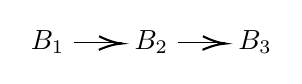
\begin{tikzpicture}[x=0.75pt,y=0.75pt,yscale=-1,xscale=1]
%uncomment if require: \path (0,797); %set diagram left start at 0, and has height of 797


% Text Node
\draw (380,0) node [anchor=north west][inner sep=0.75pt]    {$B_{1}$};
% Text Node
\onslide<4->{\draw (430,0) node [anchor=north west][inner sep=0.75pt]    {$B_{2}$};}
% Text Node
\onslide<5->{\draw (480,0) node [anchor=north west][inner sep=0.75pt]    {$B_{3}$};}
% Connection
\onslide<4->{\draw    (402,7) -- (425,7) ;
\draw [shift={(425,7.4)}, rotate = 181.36] [color={rgb, 255:red, 0; green, 0; blue, 0 }  ][line width=0.75]    (10.93,-3.29) .. controls (6.95,-1.4) and (3.31,-0.3) .. (0,0) .. controls (3.31,0.3) and (6.95,1.4) .. (10.93,3.29)   ;}
% Connection
\onslide<5->{\draw    (452,7) -- (475,7) ;
\draw [shift={(475,7.4)}, rotate = 181.4] [color={rgb, 255:red, 0; green, 0; blue, 0 }  ][line width=0.75]    (10.93,-3.29) .. controls (6.95,-1.4) and (3.31,-0.3) .. (0,0) .. controls (3.31,0.3) and (6.95,1.4) .. (10.93,3.29)   ;}

\end{tikzpicture}
\par
% \small $G$, suppose $\law \equiv \nicefrac{1}{2}$.
\end{column}
\end{columns}\pause\pause\pause

\only<6-8>{\vspace{1.5em}\centering


\tikzset{every picture/.style={line width=0.75pt}} %set default line width to 0.75pt        

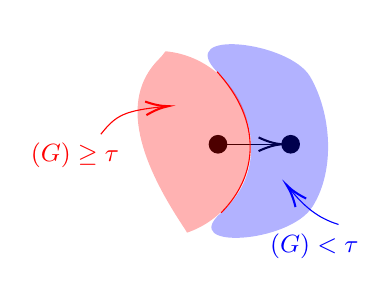
\begin{tikzpicture}[x=0.75pt,y=0.75pt,yscale=-1,xscale=1]
%uncomment if require: \path (0,797); %set diagram left start at 0, and has height of 797

\draw  [draw opacity=0][fill={rgb, 255:red, 0; green, 0; blue, 0 }  ,fill opacity=1 ][line width=0.75]  (496.6,610.1) .. controls (496.6,607.61) and (498.61,605.6) .. (501.1,605.6) .. controls (503.59,605.6) and (505.6,607.61) .. (505.6,610.1) .. controls (505.6,612.59) and (503.59,614.6) .. (501.1,614.6) .. controls (498.61,614.6) and (496.6,612.59) .. (496.6,610.1) -- cycle ;
%Shape: Circle [id:dp40521627665044346] 
\onslide<7->{\draw  [draw opacity=0][fill={rgb, 255:red, 0; green, 0; blue, 0 }  ,fill opacity=1 ][line width=0.75]  (531.6,610.1) .. controls (531.6,607.61) and (533.61,605.6) .. (536.1,605.6) .. controls (538.59,605.6) and (540.6,607.61) .. (540.6,610.1) .. controls (540.6,612.59) and (538.59,614.6) .. (536.1,614.6) .. controls (533.61,614.6) and (531.6,612.59) .. (531.6,610.1) -- cycle ;}
%Straight Lines [id:da7845811693503539] 
\onslide<7->{\draw    (505.6,610.1) -- (529.6,610.1) ;
\draw [shift={(531.6,610.1)}, rotate = 180] [color={rgb, 255:red, 0; green, 0; blue, 0 }  ][line width=0.75]    (10.93,-3.29) .. controls (6.95,-1.4) and (3.31,-0.3) .. (0,0) .. controls (3.31,0.3) and (6.95,1.4) .. (10.93,3.29)   ;}
\onslide<8->{%Shape: Path Data [id:dp33471174830726835] 
\draw  [draw opacity=0][fill={rgb, 255:red, 255; green, 0; blue, 0 }  ,fill opacity=0.3 ] (516.6,610.1) .. controls (516.6,629.85) and (503.88,646.63) .. (486.18,652.69) .. controls (485.73,651.87) and (485.21,651.01) .. (484.6,650.1) .. controls (464.6,620.1) and (452.6,589.1) .. (472.6,569.1) .. controls (474.01,567.69) and (475.06,566.42) .. (475.78,565.29) .. controls (498.67,567.4) and (516.6,586.66) .. (516.6,610.1) -- cycle ;
%Shape: Polygon Curved [id:ds8534078006559433] 
\draw  [draw opacity=0][fill={rgb, 255:red, 0; green, 0; blue, 255 }  ,fill opacity=0.3 ] (500.6,575.1) .. controls (480.07,554.2) and (535.53,560.4) .. (545.53,577.6) .. controls (555.53,594.8) and (557.93,622) .. (546.73,640) .. controls (535.53,658) and (481.93,661.2) .. (502.6,643.1) .. controls (523.27,625) and (521.13,596) .. (500.6,575.1) -- cycle ;
Shape: Circle [id:dp6323258260851117] 
%Curve Lines [id:da49729789960688] 
\draw [color={rgb, 255:red, 255; green, 0; blue, 0 }  ,draw opacity=1 ]   (500.6,575.1) .. controls (522.6,599.1) and (520.6,625.1) .. (502.6,643.1) ;
%Curve Lines [id:da9781828675291866] 
\draw [color={rgb, 255:red, 255; green, 0; blue, 0 }  ,draw opacity=1 ]   (444.67,605.25) .. controls (451.94,596.04) and (455.92,593.88) .. (475.32,591.93) ;
\draw [shift={(477.17,591.75)}, rotate = 174.56] [color={rgb, 255:red, 255; green, 0; blue, 0 }  ,draw opacity=1 ][line width=0.75]    (10.93,-3.29) .. controls (6.95,-1.4) and (3.31,-0.3) .. (0,0) .. controls (3.31,0.3) and (6.95,1.4) .. (10.93,3.29)   ;
%Curve Lines [id:da9665845518826721] 
\draw [color={rgb, 255:red, 0; green, 0; blue, 255 }  ,draw opacity=1 ]   (559.17,648.75) .. controls (549.13,645.63) and (542.82,640.32) .. (535.36,631.22) ;
\draw [shift={(534.17,629.75)}, rotate = 51.34] [color={rgb, 255:red, 0; green, 0; blue, 255 }  ,draw opacity=1 ][line width=0.75]    (10.93,-3.29) .. controls (6.95,-1.4) and (3.31,-0.3) .. (0,0) .. controls (3.31,0.3) and (6.95,1.4) .. (10.93,3.29)   ;

% Text Node
\draw (409.67,608) node [anchor=north west][inner sep=0.75pt]  [font=\small,color={rgb, 255:red, 255; green, 0; blue, 0 }  ,opacity=1 ]  {$\w(G) \geq \tau $};
% Text Node
\draw (525,652) node [anchor=north west][inner sep=0.75pt]  [font=\small,color={rgb, 255:red, 0; green, 0; blue, 255 }  ,opacity=1 ]  {$\w(G) < \tau $};}


\end{tikzpicture}
}\pause\pause\pause

\vspace{0.4em}\begin{columns}[T]
\begin{column}{.5\textwidth}
\onslide<9->{For a threshold $\tau \in [0,1]$, \begin{itemize}
    \item let $\L \subseteq \only<-11>{\G}\only<12->{\C}$ be the set of \b{likely} witness DAGs, $\w(G) \geq \tau$\only<10->{;
    \item let $\U \subseteq \only<-11>{\G}\only<12->{\C}$ be the set of \b{(most likely) unlikely} witness DAGs, $\w(G) < \tau$ such that all strict prefixes are likely.}
\end{itemize}}
\end{column}
\begin{column}{.4\textwidth}
\onslide<9->{\vspace{-0.75em}\centering


\tikzset{every picture/.style={line width=0.75pt}} %set default line width to 0.75pt        

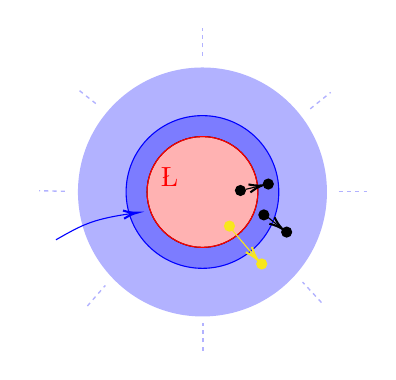
\begin{tikzpicture}[x=0.75pt,y=0.75pt,yscale=-1,xscale=1,scale=0.6]
%uncomment if require: \path (0,893); %set diagram left start at 0, and has height of 893

%Shape: Circle [id:dp6347747926336691] 
\draw  [draw opacity=0][fill={rgb, 255:red, 0; green, 0; blue, 255 }  ,fill opacity=0.3 ] (185.73,741.1) .. controls (185.73,685.89) and (230.49,641.13) .. (285.7,641.13) .. controls (340.91,641.13) and (385.67,685.89) .. (385.67,741.1) .. controls (385.67,796.31) and (340.91,841.07) .. (285.7,841.07) .. controls (230.49,841.07) and (185.73,796.31) .. (185.73,741.1) -- cycle ;
%Shape: Circle [id:dp16773685093033808] 
\onslide<10->{\draw  [color={rgb, 255:red, 0; green, 0; blue, 255 }  ,draw opacity=1 ][fill={rgb, 255:red, 0; green, 0; blue, 255 }  ,fill opacity=0.3 ] (224.39,741.1) .. controls (224.39,707.24) and (251.84,679.79) .. (285.7,679.79) .. controls (319.56,679.79) and (347.01,707.24) .. (347.01,741.1) .. controls (347.01,774.96) and (319.56,802.41) .. (285.7,802.41) .. controls (251.84,802.41) and (224.39,774.96) .. (224.39,741.1) -- cycle ;}
%Shape: Circle [id:dp86831620873002] 
\draw  [fill={rgb, 255:red, 255; green, 255; blue, 255 }  ,fill opacity=1 ] (241.2,741.1) .. controls (241.2,716.52) and (261.12,696.6) .. (285.7,696.6) .. controls (310.28,696.6) and (330.2,716.52) .. (330.2,741.1) .. controls (330.2,765.68) and (310.28,785.6) .. (285.7,785.6) .. controls (261.12,785.6) and (241.2,765.68) .. (241.2,741.1) -- cycle ;
%Shape: Circle [id:dp09468292282767443] 
\draw  [color={rgb, 255:red, 255; green, 0; blue, 0 }  ,draw opacity=1 ][fill={rgb, 255:red, 255; green, 0; blue, 0 }  ,fill opacity=0.3 ] (241.2,741.1) .. controls (241.2,716.52) and (261.12,696.6) .. (285.7,696.6) .. controls (310.28,696.6) and (330.2,716.52) .. (330.2,741.1) .. controls (330.2,765.68) and (310.28,785.6) .. (285.7,785.6) .. controls (261.12,785.6) and (241.2,765.68) .. (241.2,741.1) -- cycle ;
%Shape: Circle [id:dp9845956832929754] 
\draw  [draw opacity=0][fill={rgb, 255:red, 0; green, 0; blue, 0 }  ,fill opacity=1 ][line width=0.75]  (311.7,739.9) .. controls (311.7,737.41) and (313.71,735.4) .. (316.2,735.4) .. controls (318.69,735.4) and (320.7,737.41) .. (320.7,739.9) .. controls (320.7,742.39) and (318.69,744.4) .. (316.2,744.4) .. controls (313.71,744.4) and (311.7,742.39) .. (311.7,739.9) -- cycle ;
%Shape: Circle [id:dp7570400850625347] 
\draw  [draw opacity=0][fill={rgb, 255:red, 0; green, 0; blue, 0 }  ,fill opacity=1 ][line width=0.75]  (334.07,734.73) .. controls (334.07,732.25) and (336.08,730.23) .. (338.57,730.23) .. controls (341.05,730.23) and (343.07,732.25) .. (343.07,734.73) .. controls (343.07,737.22) and (341.05,739.23) .. (338.57,739.23) .. controls (336.08,739.23) and (334.07,737.22) .. (334.07,734.73) -- cycle ;
%Straight Lines [id:da4946555213004382] 
\draw    (320.7,738.9) -- (332.12,736.19) ;
\draw [shift={(334.07,735.73)}, rotate = 166.67] [color={rgb, 255:red, 0; green, 0; blue, 0 }  ][line width=0.75]    (10.93,-3.29) .. controls (6.95,-1.4) and (3.31,-0.3) .. (0,0) .. controls (3.31,0.3) and (6.95,1.4) .. (10.93,3.29)   ;
\onslide<10->{%Shape: Circle [id:dp21475200286126772] 
\draw  [draw opacity=0][fill={rgb, 255:red, 0; green, 0; blue, 0 }  ,fill opacity=1 ][line width=0.75]  (330.5,759.5) .. controls (330.5,757.01) and (332.51,755) .. (335,755) .. controls (337.49,755) and (339.5,757.01) .. (339.5,759.5) .. controls (339.5,761.99) and (337.49,764) .. (335,764) .. controls (332.51,764) and (330.5,761.99) .. (330.5,759.5) -- cycle ;
%Shape: Circle [id:dp6401125405786658] 
\draw  [draw opacity=0][fill={rgb, 255:red, 0; green, 0; blue, 0 }  ,fill opacity=1 ][line width=0.75]  (348.8,773.3) .. controls (348.8,770.81) and (350.81,768.8) .. (353.3,768.8) .. controls (355.79,768.8) and (357.8,770.81) .. (357.8,773.3) .. controls (357.8,775.79) and (355.79,777.8) .. (353.3,777.8) .. controls (350.81,777.8) and (348.8,775.79) .. (348.8,773.3) -- cycle ;
%Straight Lines [id:da6137452163851853] 
\draw    (337.67,760.93) -- (348.44,769.64) ;
\draw [shift={(350,770.9)}, rotate = 218.94] [color={rgb, 255:red, 0; green, 0; blue, 0 }  ][line width=0.75]    (10.93,-3.29) .. controls (6.95,-1.4) and (3.31,-0.3) .. (0,0) .. controls (3.31,0.3) and (6.95,1.4) .. (10.93,3.29)   ;}
%Shape: Circle [id:dp4856749631522035] 
\onslide<11->{\draw  [draw opacity=0][fill={rgb, 255:red, 248; green, 231; blue, 28 }  ,fill opacity=1 ][line width=0.75]  (302.9,768.5) .. controls (302.9,766.01) and (304.91,764) .. (307.4,764) .. controls (309.89,764) and (311.9,766.01) .. (311.9,768.5) .. controls (311.9,770.99) and (309.89,773) .. (307.4,773) .. controls (304.91,773) and (302.9,770.99) .. (302.9,768.5) -- cycle ;
%Shape: Circle [id:dp8734179708310015] 
\draw  [draw opacity=0][fill={rgb, 255:red, 248; green, 231; blue, 28 }  ,fill opacity=1 ][line width=0.75]  (328.8,798.9) .. controls (328.8,796.41) and (330.81,794.4) .. (333.3,794.4) .. controls (335.79,794.4) and (337.8,796.41) .. (337.8,798.9) .. controls (337.8,801.39) and (335.79,803.4) .. (333.3,803.4) .. controls (330.81,803.4) and (328.8,801.39) .. (328.8,798.9) -- cycle ;
%Straight Lines [id:da3880974951160452] 
\draw [color={rgb, 255:red, 248; green, 231; blue, 28 }  ,draw opacity=1 ][fill={rgb, 255:red, 155; green, 155; blue, 155 }  ,fill opacity=1 ]   (309.67,771.73) -- (328.77,794.21) ;
\draw [shift={(330.07,795.73)}, rotate = 229.64] [color={rgb, 255:red, 248; green, 231; blue, 28 }  ,draw opacity=1 ][line width=0.75]    (10.93,-3.29) .. controls (6.95,-1.4) and (3.31,-0.3) .. (0,0) .. controls (3.31,0.3) and (6.95,1.4) .. (10.93,3.29)   ;}
%Straight Lines [id:da5165162315025413] 
\draw [color={rgb, 255:red, 0; green, 0; blue, 255 }  ,draw opacity=0.3 ][line width=0.5]  [dash pattern={on 1.5pt off 1.5pt}]  (395.07,740.53) -- (417.87,740.53) ;
%Straight Lines [id:da38753837989284445] 
\draw [color={rgb, 255:red, 0; green, 0; blue, 255 }  ,draw opacity=0.3 ][line width=0.5]  [dash pattern={on 1.5pt off 1.5pt}]  (372.27,674.33) -- (388.67,661.13) ;
%Straight Lines [id:da007919123820054441] 
\draw [color={rgb, 255:red, 0; green, 0; blue, 255 }  ,draw opacity=0.3 ][line width=0.5]  [dash pattern={on 1.5pt off 1.5pt}]  (285.67,631.73) -- (285.67,609.73) ;
%Straight Lines [id:da7968663560498248] 
\draw [color={rgb, 255:red, 0; green, 0; blue, 255 }  ,draw opacity=0.3 ][line width=0.5]  [dash pattern={on 1.5pt off 1.5pt}]  (200.07,670.13) -- (184.47,657.73) ;
%Straight Lines [id:da48757360196126287] 
\draw [color={rgb, 255:red, 0; green, 0; blue, 255 }  ,draw opacity=0.3 ][line width=0.5]  [dash pattern={on 1.5pt off 1.5pt}]  (175.27,740.53) -- (154.47,740.13) ;
%Straight Lines [id:da11971479686666275] 
\draw [color={rgb, 255:red, 0; green, 0; blue, 255 }  ,draw opacity=0.3 ][line width=0.5]  [dash pattern={on 1.5pt off 1.5pt}]  (286.07,868.53) -- (286.07,846.53) ;
%Straight Lines [id:da6484236736378048] 
\draw [color={rgb, 255:red, 0; green, 0; blue, 255 }  ,draw opacity=0.3 ][line width=0.5]  [dash pattern={on 1.5pt off 1.5pt}]  (381.27,829.88) -- (366.07,813.39) ;
%Straight Lines [id:da25336093141802474] 
\draw [color={rgb, 255:red, 0; green, 0; blue, 255 }  ,draw opacity=0.3 ][line width=0.5]  [dash pattern={on 1.5pt off 1.5pt}]  (193.27,832.68) -- (207.67,816.19) ;
%Curve Lines [id:da46026392802664984] 
\onslide<10->{\draw [color={rgb, 255:red, 0; green, 0; blue, 255 }  ,draw opacity=1 ]   (168.07,779.48) .. controls (190.92,766.47) and (197.86,762.79) .. (231.61,757.97) ;
\draw [shift={(233.17,757.75)}, rotate = 172.01] [color={rgb, 255:red, 0; green, 0; blue, 255 }  ,draw opacity=1 ][line width=0.75]    (10.93,-3.29) .. controls (6.95,-1.4) and (3.31,-0.3) .. (0,0) .. controls (3.31,0.3) and (6.95,1.4) .. (10.93,3.29)   ;}

% Text Node
\draw (250.2,719.6) node [anchor=north west][inner sep=0.75pt]  [color={rgb, 255:red, 255; green, 0; blue, 0 }  ,opacity=1 ]  {$\L$};
% Text Node
\onslide<10->{\draw (145.8,774) node [anchor=north west][inner sep=0.75pt]  [color={rgb, 255:red, 0; green, 0; blue, 255 }  ,opacity=1 ]  {$\U$};}


\end{tikzpicture}
}
\end{column}
\end{columns}\pause\pause\pause

% Idea: choose $R$ such that unlikely resamples are avoided!

% \begin{columns}[T]
% \begin{column}{.55\textwidth}
% \g{Example}\quad $\w(G) = \only<2-3>{\nicefrac{1}{4}}\only<4>{\nicefrac{1}{16}}\only<5->{\nicefrac{1}{32}}$.\vspace{0.3em}

% \onslide<6->{For a threshold $\tau \in [0,1]$, \begin{itemize}
%     \item let $\L \subseteq \only<-8>{\G}\only<9->{\C}$ be the set of \b{likely} witness DAGs, $\w(G) \geq \tau$\only<7->{;
%     \item let $\U \subseteq \only<-8>{\G}\only<9->{\C}$ be the set of \b{(most likely) unlikely} witness DAGs, $\w(G) < \tau$ such that all strict prefixes are likely.}
% \end{itemize}}

% \onslide<8->{\underline{Problem}: $\U$ does not form a complete boundary of $\L$!}
% \end{column}
% \begin{column}{.36\textwidth}
% \centering


\tikzset{every picture/.style={line width=0.75pt}} %set default line width to 0.75pt        

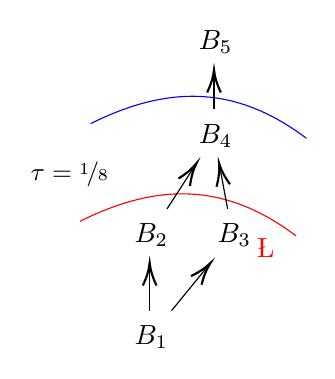
\begin{tikzpicture}[x=0.75pt,y=0.75pt,yscale=-1,xscale=1]
%uncomment if require: \path (0,534); %set diagram left start at 0, and has height of 534

%Curve Lines [id:da3428774655789326] 
\onslide<6->{\draw [color={rgb, 255:red, 255; green, 0; blue, 0 }  ,draw opacity=1 ]   (253,380) .. controls (293,360) and (325,363) .. (357,387) ;}
%Curve Lines [id:da41651271023154823] 
\onslide<7->{\draw [color={rgb, 255:red, 0; green, 0; blue, 255 }  ,draw opacity=1 ]   (258,333) .. controls (298,313) and (330,316) .. (362,340) ;}

% Text Node
\onslide<2,4->{\draw (278,380) node [anchor=north west][inner sep=0.75pt]    {$B_{2}$};}
\onslide<3>{\draw (278,380) node [anchor=north west][inner sep=0.75pt] [opacity=0.2  ]    {$B_{2}$};}
% Text Node
\onslide<4->{\draw (309,332) node [anchor=north west][inner sep=0.75pt]    {$B_{4}$};}
\onslide<2-3>{\draw (309,332) node [anchor=north west][inner sep=0.75pt] [opacity=0.2  ]    {$B_{4}$};}
% Text Node
\draw (278,429) node [anchor=north west][inner sep=0.75pt]    {$B_{1}$};
% Text Node
\onslide<3->{\draw (318,380) node [anchor=north west][inner sep=0.75pt]    {$B_{3}$};}
\onslide<2>{\draw (318,380) node [anchor=north west][inner sep=0.75pt] [opacity=0.2  ]    {$B_{3}$};}
% Text Node
\onslide<5->{\draw (309,287) node [anchor=north west][inner sep=0.75pt]    {$B_{5}$};}
\onslide<2-4>{\draw (309,287) node [anchor=north west][inner sep=0.75pt] [opacity=0.2  ]    {$B_{5}$};}
% Connection 1
\onslide<2,4->{\draw    (286.5,402) -- (286.5,423) ;
\draw [shift={(286.5,400)}, rotate = 90] [color={rgb, 255:red, 0; green, 0; blue, 0 }  ][line width=0.75]    (10.93,-3.29) .. controls (6.95,-1.4) and (3.31,-0.3) .. (0,0) .. controls (3.31,0.3) and (6.95,1.4) .. (10.93,3.29)   ;}
\onslide<3>{\draw [opacity=0.2  ]    (286.5,402) -- (286.5,423) ;
\draw [shift={(286.5,400)}, rotate = 90] [color={rgb, 255:red, 0; green, 0; blue, 0 },opacity=0.2  ][line width=0.75]    (10.93,-3.29) .. controls (6.95,-1.4) and (3.31,-0.3) .. (0,0) .. controls (3.31,0.3) and (6.95,1.4) .. (10.93,3.29)   ;}
% Connection 3
\onslide<4->{\draw    (294.9,374) -- (308.02,353.68) ;
\draw [shift={(309.1,352)}, rotate = 122.86] [color={rgb, 255:red, 0; green, 0; blue, 0 }  ][line width=0.75]    (10.93,-3.29) .. controls (6.95,-1.4) and (3.31,-0.3) .. (0,0) .. controls (3.31,0.3) and (6.95,1.4) .. (10.93,3.29)   ;}
\onslide<2-3>{\draw [opacity=0.2  ]    (294.9,374) -- (308.02,353.68) ;
\draw [shift={(309.1,352)}, rotate = 122.86] [color={rgb, 255:red, 0; green, 0; blue, 0 },opacity=0.2  ][line width=0.75]    (10.93,-3.29) .. controls (6.95,-1.4) and (3.31,-0.3) .. (0,0) .. controls (3.31,0.3) and (6.95,1.4) .. (10.93,3.29)   ;}
% Connection 4
\onslide<4->{\draw    (324.06,374) -- (320.31,353.97) ;
\draw [shift={(319.94,352)}, rotate = 79.38] [color={rgb, 255:red, 0; green, 0; blue, 0 }  ][line width=0.75]    (10.93,-3.29) .. controls (6.95,-1.4) and (3.31,-0.3) .. (0,0) .. controls (3.31,0.3) and (6.95,1.4) .. (10.93,3.29)   ;}
\onslide<2-3>{\draw [opacity=0.2  ]    (324.06,374) -- (320.31,353.97) ;
\draw [shift={(319.94,352)}, rotate = 79.38] [color={rgb, 255:red, 0; green, 0; blue, 0 },opacity=0.2  ][line width=0.75]    (10.93,-3.29) .. controls (6.95,-1.4) and (3.31,-0.3) .. (0,0) .. controls (3.31,0.3) and (6.95,1.4) .. (10.93,3.29)   ;}
% Connection 2
\onslide<3->{\draw    (297.11,423) -- (314.62,401.55) ;
\draw [shift={(315.89,400)}, rotate = 129.23] [color={rgb, 255:red, 0; green, 0; blue, 0 }  ][line width=0.75]    (10.93,-3.29) .. controls (6.95,-1.4) and (3.31,-0.3) .. (0,0) .. controls (3.31,0.3) and (6.95,1.4) .. (10.93,3.29)   ;}
\onslide<2>{\draw [opacity=0.2  ]    (297.11,423) -- (314.62,401.55) ;
\draw [shift={(315.89,400)}, rotate = 129.23] [color={rgb, 255:red, 0; green, 0; blue, 0 },opacity=0.2  ][line width=0.75]    (10.93,-3.29) .. controls (6.95,-1.4) and (3.31,-0.3) .. (0,0) .. controls (3.31,0.3) and (6.95,1.4) .. (10.93,3.29)   ;}
% Connection 5
\onslide<5->{\draw    (317.5,326) -- (317.5,309) ;
\draw [shift={(317.5,307)}, rotate = 90] [color={rgb, 255:red, 0; green, 0; blue, 0 }  ][line width=0.75]    (10.93,-3.29) .. controls (6.95,-1.4) and (3.31,-0.3) .. (0,0) .. controls (3.31,0.3) and (6.95,1.4) .. (10.93,3.29)   ;}
\onslide<2-4>{\draw [opacity=0.2  ]    (317.5,326) -- (317.5,309) ;
\draw [shift={(317.5,307)}, rotate = 90] [color={rgb, 255:red, 0; green, 0; blue, 0 },opacity=0.2  ][line width=0.75]    (10.93,-3.29) .. controls (6.95,-1.4) and (3.31,-0.3) .. (0,0) .. controls (3.31,0.3) and (6.95,1.4) .. (10.93,3.29)   ;}

% \draw (250,287) node [anchor=north west][inner sep=0.75pt]    {$G$};

% Text Node
\onslide<6->{\draw (228,350) node [anchor=north west][inner sep=0.75pt]  [font=\small,color={rgb, 255:red, 0; green, 0; blue, 0 }  ,opacity=1 ]  {$\tau =\nicefrac{1}{8}$};}

% Text Node
\onslide<6->{\draw (337,387) node [anchor=north west][inner sep=0.75pt]  [color={rgb, 255:red, 255; green, 0; blue, 0 }  ,opacity=1 ]  {$\L$};}
% Text Node
\onslide<7->{\draw (335,338) node [anchor=north west][inner sep=0.75pt]  [color={rgb, 255:red, 0; green, 0; blue, 255 }  ,opacity=1 ]  {$\U$};}

\end{tikzpicture}

% \flushright\small $G$, suppose $\law \equiv \nicefrac{1}{2}$.
% \end{column}
% \end{columns}\vspace{0.25em}\pause\pause\pause\pause\pause\pause\pause

% Consider the larger set $\C$ of all witness DAGs attainable by removing the sink of some single-sink witness DAG \follows $\G \subseteq \C$.\pause\spadding

Need to consider all witness DAGs attainable by removing the sink of some single-sink witness DAG (set denoted $\C$).\pause

\follows fixing resampling table $R$, if $\compat{\U}{R} = \emptyset$, then $\compat{\C}{R} \subseteq \compat{\L}{R}$.
\end{frame}

\begin{frame}{Finding Resampling Table avoiding $\U$}
Using the method of conditional expectation, we find $R$ such that \vspace{-0.5em}\begin{align*}
    |\compat{\U}{R}| \leq \E[R \sim \distr]{|\compat{\U}{R}|} \pause = \w(\U).
\end{align*}\pause

\vspace{-1.8em}\follows if we choose $\tau$ such that $\w(\U) < 1$,\par then $\compat{\U}{R} = \emptyset$ and $\compat{\G}{R} \subseteq \compat{\L}{R}$.\pause\padding

What is the effect of changing $\tau$?\pause\vspace{0.1em}

\centering


\tikzset{every picture/.style={line width=0.75pt}} %set default line width to 0.75pt        

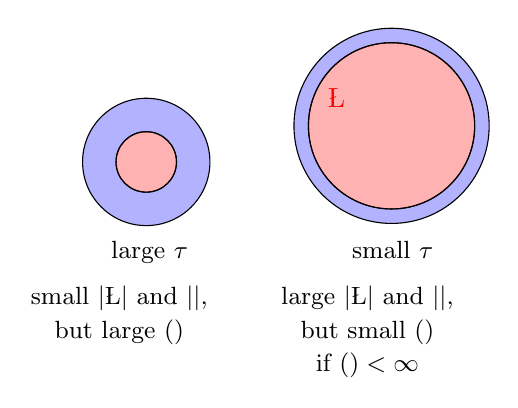
\begin{tikzpicture}[x=0.75pt,y=0.75pt,yscale=-1,xscale=1,scale=0.9]
%uncomment if require: \path (0,797); %set diagram left start at 0, and has height of 797

%Shape: Circle [id:dp7800027250553745] 
\draw  [fill={rgb, 255:red, 0; green, 0; blue, 255 }  ,fill opacity=0.3 ] (262.25,535.5) .. controls (262.25,506.64) and (285.64,483.25) .. (314.5,483.25) .. controls (343.36,483.25) and (366.75,506.64) .. (366.75,535.5) .. controls (366.75,564.36) and (343.36,587.75) .. (314.5,587.75) .. controls (285.64,587.75) and (262.25,564.36) .. (262.25,535.5) -- cycle ;
%Shape: Circle [id:dp4478372855789199] 
\draw  [fill={rgb, 255:red, 255; green, 255; blue, 255 }  ,fill opacity=1 ] (270,535.5) .. controls (270,510.92) and (289.92,491) .. (314.5,491) .. controls (339.08,491) and (359,510.92) .. (359,535.5) .. controls (359,560.08) and (339.08,580) .. (314.5,580) .. controls (289.92,580) and (270,560.08) .. (270,535.5) -- cycle ;
%Shape: Circle [id:dp48307643021971036] 
\draw  [fill={rgb, 255:red, 255; green, 0; blue, 0 }  ,fill opacity=0.3 ] (270,535.5) .. controls (270,510.92) and (289.92,491) .. (314.5,491) .. controls (339.08,491) and (359,510.92) .. (359,535.5) .. controls (359,560.08) and (339.08,580) .. (314.5,580) .. controls (289.92,580) and (270,560.08) .. (270,535.5) -- cycle ;

%Shape: Circle [id:dp11789160769727891] 
\draw  [fill={rgb, 255:red, 0; green, 0; blue, 255 }  ,fill opacity=0.3 ] (149.09,554.82) .. controls (149.09,535.99) and (164.35,520.73) .. (183.18,520.73) .. controls (202.01,520.73) and (217.27,535.99) .. (217.27,554.82) .. controls (217.27,573.65) and (202.01,588.91) .. (183.18,588.91) .. controls (164.35,588.91) and (149.09,573.65) .. (149.09,554.82) -- cycle ;
%Shape: Circle [id:dp25526749807152616] 
\draw  [fill={rgb, 255:red, 255; green, 255; blue, 255 }  ,fill opacity=1 ] (167,554.82) .. controls (167,545.88) and (174.25,538.63) .. (183.18,538.63) .. controls (192.12,538.63) and (199.37,545.88) .. (199.37,554.82) .. controls (199.37,563.75) and (192.12,571) .. (183.18,571) .. controls (174.25,571) and (167,563.75) .. (167,554.82) -- cycle ;
%Shape: Circle [id:dp4162737382136239] 
\draw  [fill={rgb, 255:red, 255; green, 0; blue, 0 }  ,fill opacity=0.3 ] (167,554.82) .. controls (167,545.88) and (174.25,538.63) .. (183.18,538.63) .. controls (192.12,538.63) and (199.37,545.88) .. (199.37,554.82) .. controls (199.37,563.75) and (192.12,571) .. (183.18,571) .. controls (174.25,571) and (167,563.75) .. (167,554.82) -- cycle ;


% Text Node
\draw (279,514) node [anchor=north west][inner sep=0.75pt]  [color={rgb, 255:red, 255; green, 0; blue, 0 }  ,opacity=1 ]  {$\L$};
% Text Node
\draw (246,496) node [anchor=north west][inner sep=0.75pt]  [color={rgb, 255:red, 0; green, 0; blue, 255 }  ,opacity=1 ]  {\U};
% Text Node
\draw (163,596) node [anchor=north west][inner sep=0.75pt]   [align=left] {\small large $\displaystyle \tau $};
% Text Node
\onslide<6->{\draw (120,620) node [anchor=north west][inner sep=0.75pt]   [align=center] {\small small $|\L|$ and $|\U|$,\\\small but large $\w(\U)$};}
% Text Node
\draw (292,596) node [anchor=north west][inner sep=0.75pt]   [align=left] {\small small $\displaystyle \tau $};
% Text Node
\onslide<7->{\draw (254,620) node [anchor=north west][inner sep=0.75pt]   [align=center] {\small large $|\L|$ and $|\U|$,\\\small but small $\w(\U)$ \\\small if $\w(\C) < \infty$};}


\end{tikzpicture}

\end{frame}

\begin{frame}{Choosing the Threshold}
Can we choose $\tau$ such that $\w(\U) < 1$ and $\U$ and $\L$ are of polynomial size?\pause

What is the largest $\tau$ guaranteeing $\w(\U) < 1$?\pause\spadding
    
% We compare $\w$ and $\epsw$.\pause\par
% For $G \in \U$, suppose $\epsw(G) < \tau$.\pause\par
% Then, $\w(G) < \tau^\epsilon \epsw(G)$\pause\ \follows $\w(\U) < \tau^\epsilon \epsw(\U)$.\pause\par
$\w(G) = \epsw(G)^{\frac{1}{1-\epsilon}} \pause= \epsw(G)^{1+\epsilon'} = {\uncoverubrace<5->{\epsw(G)}{\ensuremath{< \tau}}}^{\epsilon'} \epsw(G)$.\pause\par
\vspace{-1.3em}\follows $\w(\U) < \tau^{\epsilon'} \epsw(\U)$.\pause\par
\follows for $\tau \leq \taumax$, we have $\w(\U) < 1$.\pause

% % wiggle proportional to weight of object (if weight of object depends on \tau, wiggle depends on \tau)    
% 


\tikzset{every picture/.style={line width=0.75pt}} %set default line width to 0.75pt        

\begin{tikzpicture}[remember picture,overlay]
\node[left,xshift=-2em,yshift=-7em] at (current page.north east){%
    \begin{tikzpicture}[x=0.75pt,y=0.75pt,yscale=-1,xscale=1,scale=0.75]
    %uncomment if require: \path (0,534); %set diagram left start at 0, and has height of 534
    
    %Shape: Circle [id:dp4449959236715497] 
    \draw  [fill={rgb, 255:red, 0; green, 0; blue, 0 }  ,fill opacity=0.2 ] (483.5,334) .. controls (483.5,314.12) and (499.62,298) .. (519.5,298) .. controls (539.38,298) and (555.5,314.12) .. (555.5,334) .. controls (555.5,353.88) and (539.38,370) .. (519.5,370) .. controls (499.62,370) and (483.5,353.88) .. (483.5,334) -- cycle ;
    %Shape: Circle [id:dp814318525383303] 
    \draw  [fill={rgb, 255:red, 0; green, 0; blue, 0 }  ,fill opacity=0.2 ] (443.68,353) .. controls (443.68,343.61) and (451.29,336) .. (460.68,336) .. controls (470.07,336) and (477.68,343.61) .. (477.68,353) .. controls (477.68,362.39) and (470.07,370) .. (460.68,370) .. controls (451.29,370) and (443.68,362.39) .. (443.68,353) -- cycle ;
    
    % %Shape: Circle [id:dp4449959236715497] 
    % \draw  [fill={rgb, 255:red, 0; green, 0; blue, 0 }  ,fill opacity=0.2 ] (503,343.5) .. controls (503,328.86) and (514.86,317) .. (529.5,317) .. controls (544.14,317) and (556,328.86) .. (556,343.5) .. controls (556,358.14) and (544.14,370) .. (529.5,370) .. controls (514.86,370) and (503,358.14) .. (503,343.5) -- cycle ;
    %Shape: Circle [id:dp34202212243960495] 
    \draw  [fill={rgb, 255:red, 0; green, 0; blue, 0 }  ,fill opacity=1 ] (493,343.5) .. controls (493,328.86) and (504.86,317) .. (519.5,317) .. controls (534.14,317) and (546,328.86) .. (546,343.5) .. controls (546,358.14) and (534.14,370) .. (519.5,370) .. controls (504.86,370) and (493,358.14) .. (493,343.5) -- cycle ;
    % %Shape: Circle [id:dp814318525383303] 
    % \draw  [fill={rgb, 255:red, 0; green, 0; blue, 0 }  ,fill opacity=0.2 ] (452.79,357.32) .. controls (452.79,350.31) and (458.46,344.63) .. (465.47,344.63) .. controls (472.47,344.63) and (478.15,350.31) .. (478.15,357.32) .. controls (478.15,364.32) and (472.47,370) .. (465.47,370) .. controls (458.46,370) and (452.79,364.32) .. (452.79,357.32) -- cycle ;
    %Shape: Circle [id:dp5272256995859699] 
    \draw  [fill={rgb, 255:red, 0; green, 0; blue, 0 }  ,fill opacity=1 ] (448,357.32) .. controls (448,350.31) and (453.68,344.63) .. (460.68,344.63) .. controls (467.69,344.63) and (473.37,350.31) .. (473.37,357.32) .. controls (473.37,364.32) and (467.69,370) .. (460.68,370) .. controls (453.68,370) and (448,364.32) .. (448,357.32) -- cycle ;
    
    % Text Node
    \draw (507,335) node [anchor=north west][inner sep=0.75pt]  [font=\small,color={rgb, 255:red, 255; green, 255; blue, 255 }  ,opacity=1 ]  {\small$G_2$};
    % Text Node
    \draw (449,349) node [anchor=north west][inner sep=0.75pt]  [font=\small,color={rgb, 255:red, 255; green, 255; blue, 255 }  ,opacity=1 ]  {\small$G_1$};
    % Text Node
    \draw (445,375) node [anchor=north west][inner sep=0.75pt]  [font=\small,color={rgb, 255:red, 0; green, 0; blue, 0 }  ,opacity=1 ]  {\small for $G_1,G_2 \in \U$};
    
    \end{tikzpicture}
} ;
\end{tikzpicture}
\pause\vspace{-1em}

% For $G \in \U$, by how much does $\w(G)$ change\par (depending on $\tau$) when perturbing $p$?\pause\par
% We compare $\w$ and $\epsw$\pause\ \follows $\w(\U) < \tau^\epsilon \epsw(\U)$\pause\ if we choose $\U$ and $\L$ based on $\epsw$ rather than $\w$.\pause\spadding

% Need to ensure that the effect of perturbing $p$ is small enough!\pause\par
% \follows for $\tau \leq \taumax$, we have $\w(\U) < 1$.\pause
% \follows for $\tau^\epsilon \leq \epsw(\U)^{-1}$, we have $\w(\U) < 1$\pause\ \follows $\taumax$.\pause

% For $G \in \U$, we know $\w(G) < \tau$.\pause\par
% \underline{Note}: For $\epsilon > 0$, $\w(G) = \epsw(G)^{\nicefrac{1}{(1-\epsilon)}} \pause< \tau^\epsilon \epsw(G)$\par if we choose $\U$ and $\L$ based on $\epsw$ rather than $\w$\par (this we do from now on!).\pause\par
% \follows $\w(\U) < \tau^\epsilon \epsw(\U)$.\pause\par
% \follows for $\tau \leq \epsw(\U)^{-\nicefrac{1}{\epsilon}} \eqdef \taumax$, we have $\w(\U) < 1$.\pause

\vspace{0.5em}\begin{columns}[T]
\begin{column}{0.5\textwidth}
How do we compute $\tau$?\pause\par
Use exponential backoff!

\g{Example}\quad $\tau = \only<8>{2^0 = 1}\only<9>{2^{-1} = \nicefrac{1}{2}}\only<10>{2^{-2} = \nicefrac{1}{4}}\only<11->{2^{-3} = \nicefrac{1}{8}}$.\spadding%\vspace{0.25em}

% \onslide<12->{\follows $\tau \geq \frac{1}{2} \taumax$}\spadding

\onslide<12->{Are $\U$ and $\L$ of polynomial size?}
\end{column}
\begin{column}{0.3\textwidth}
\centering


\tikzset{every picture/.style={line width=0.75pt}} %set default line width to 0.75pt        

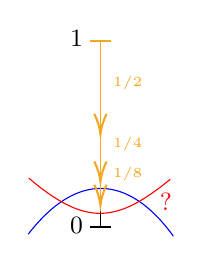
\begin{tikzpicture}[x=0.75pt,y=0.75pt,yscale=-1,xscale=1,rotate=180,scale=0.9]
%uncomment if require: \path (0,534); %set diagram left start at 0, and has height of 534

%Straight Lines [id:da8648942484395017] 
\draw    (590.4,100.4) -- (590.4,200.07) ;
\draw [shift={(590.4,200.07)}, rotate = 270] [color={rgb, 255:red, 245; green, 166; blue, 35 }  ][line width=0.75]    (0,5.59) -- (0,-5.59)   ;
\draw [shift={(590.4,100.4)}, rotate = 270] [color={rgb, 255:red, 0; green, 0; blue, 0 }  ][line width=0.75]    (0,5.59) -- (0,-5.59)   ;

% Text Node
\draw (608,107) node [anchor=north west][inner sep=0.75pt]  [font=\small]  {$0$};
% Text Node
\draw (608,207) node [anchor=north west][inner sep=0.75pt]  [font=\small]  {$1$};
% Text Node
\onslide<8->{\draw (584,102) node [anchor=north west][inner sep=0.75pt]  [font=\small,color={rgb, 255:red, 0; green, 0; blue, 255 }  ,opacity=1 ]  {$\taumax$};}
% Text Node
\onslide<9->{\draw (585,183) node [anchor=north west][inner sep=0.75pt]  [font=\footnotesize,color={rgb, 255:red, 245; green, 166; blue, 35 }  ,opacity=1 ]  {$1/2$};}
% Text Node
\onslide<10->{\draw (585,150) node [anchor=north west][inner sep=0.75pt]  [font=\footnotesize,color={rgb, 255:red, 245; green, 166; blue, 35 }  ,opacity=1 ]  {$1/4$};}
% Text Node
\onslide<11->{\draw (585,134) node [anchor=north west][inner sep=0.75pt]  [font=\footnotesize,color={rgb, 255:red, 245; green, 166; blue, 35 }  ,opacity=1 ]  {$1/8$};}
% Text Node
\onslide<12->{\draw (560,120) node [anchor=north west][inner sep=0.75pt]  [font=\small,color={rgb, 255:red, 255; green, 0; blue, 0 }  ,opacity=1 ] [align=left] {?};}

%Curve Lines [id:da5356270327996431] 
\onslide<8->{\draw [color={rgb, 255:red, 0; green, 0; blue, 255 }  ,draw opacity=1 ]   (551.4,95.73) .. controls (575.4,128.73) and (603.07,130.4) .. (629.07,96.73) ;}

%Straight Lines [id:da42007517029648045] 
\onslide<9->{\draw [color={rgb, 255:red, 245; green, 166; blue, 35 }  ,draw opacity=1 ]   (590.4,200.07) -- (590.4,152.23) ;
\draw [shift={(590.4,150.23)}, rotate = 90] [color={rgb, 255:red, 245; green, 166; blue, 35 }  ,draw opacity=1 ][line width=0.75]    (10.93,-3.29) .. controls (6.95,-1.4) and (3.31,-0.3) .. (0,0) .. controls (3.31,0.3) and (6.95,1.4) .. (10.93,3.29)   ;}
%Straight Lines [id:da4473125650369483] 
\onslide<10->{\draw [color={rgb, 255:red, 245; green, 166; blue, 35 }  ,draw opacity=1 ]   (590.4,150.23) -- (590.4,126.73) ;
\draw [shift={(590.4,124.73)}, rotate = 90] [color={rgb, 255:red, 245; green, 166; blue, 35 }  ,draw opacity=1 ][line width=0.75]    (10.93,-3.29) .. controls (6.95,-1.4) and (3.31,-0.3) .. (0,0) .. controls (3.31,0.3) and (6.95,1.4) .. (10.93,3.29)   ;}
%Straight Lines [id:da921748453412278] 
\onslide<11->{\draw [color={rgb, 255:red, 245; green, 166; blue, 35 }  ,draw opacity=1 ]   (590.4,124.73) -- (590.4,114.23) ;
\draw [shift={(590.4,112.23)}, rotate = 90] [color={rgb, 255:red, 245; green, 166; blue, 35 }  ,draw opacity=1 ][line width=0.75]    (10.93,-3.29) .. controls (6.95,-1.4) and (3.31,-0.3) .. (0,0) .. controls (3.31,0.3) and (6.95,1.4) .. (10.93,3.29)   ;}

%Curve Lines [id:da40449977786973723] 
\onslide<12->{\draw [color={rgb, 255:red, 255; green, 0; blue, 0 }  ,draw opacity=1 ]   (553.07,126.07) .. controls (581.4,103.07) and (597.73,100.4) .. (628.73,126.73) ;}


\end{tikzpicture}

\end{column}
\begin{column}{0\textwidth}
\end{column}
\end{columns}
\end{frame}

\begin{frame}{Is $\U \cup \L$ of polynomial size?}
Need to bound \# of multi-sink witness DAGs\par
and \only<1>{\# of single-sink witness DAGs}\only<2->{\underline{\# of single-sink witness DAGs}}.\pause\pause

\vspace{0.5em}\begin{center}
    


\tikzset{every picture/.style={line width=0.75pt}} %set default line width to 0.75pt        

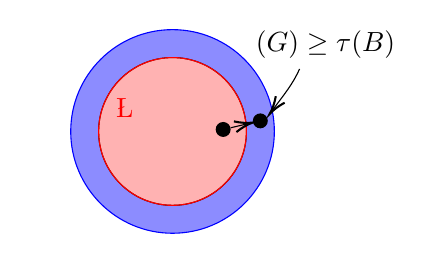
\begin{tikzpicture}[x=0.75pt,y=0.75pt,yscale=-1,xscale=1,scale=0.8]
%uncomment if require: \path (0,1301); %set diagram left start at 0, and has height of 1301

%Shape: Circle [id:dp47986660056185837] 
\draw  [color={rgb, 255:red, 0; green, 0; blue, 255 }  ,draw opacity=1 ][fill={rgb, 255:red, 0; green, 0; blue, 255 }  ,fill opacity=0.45 ] (223.39,1067.1) .. controls (223.39,1033.24) and (250.84,1005.79) .. (284.7,1005.79) .. controls (318.56,1005.79) and (346.01,1033.24) .. (346.01,1067.1) .. controls (346.01,1100.96) and (318.56,1128.41) .. (284.7,1128.41) .. controls (250.84,1128.41) and (223.39,1100.96) .. (223.39,1067.1) -- cycle ;
%Shape: Circle [id:dp35612564405295855] 
\draw  [fill={rgb, 255:red, 255; green, 255; blue, 255 }  ,fill opacity=1 ] (240.2,1067.1) .. controls (240.2,1042.52) and (260.12,1022.6) .. (284.7,1022.6) .. controls (309.28,1022.6) and (329.2,1042.52) .. (329.2,1067.1) .. controls (329.2,1091.68) and (309.28,1111.6) .. (284.7,1111.6) .. controls (260.12,1111.6) and (240.2,1091.68) .. (240.2,1067.1) -- cycle ;
%Shape: Circle [id:dp14338934667239034] 
\draw  [color={rgb, 255:red, 255; green, 0; blue, 0 }  ,draw opacity=1 ][fill={rgb, 255:red, 255; green, 0; blue, 0 }  ,fill opacity=0.3 ] (240.2,1067.1) .. controls (240.2,1042.52) and (260.12,1022.6) .. (284.7,1022.6) .. controls (309.28,1022.6) and (329.2,1042.52) .. (329.2,1067.1) .. controls (329.2,1091.68) and (309.28,1111.6) .. (284.7,1111.6) .. controls (260.12,1111.6) and (240.2,1091.68) .. (240.2,1067.1) -- cycle ;
%Shape: Circle [id:dp1521758257493362] 
\draw  [draw opacity=0][fill={rgb, 255:red, 0; green, 0; blue, 0 }  ,fill opacity=1 ][line width=0.75]  (310.7,1065.9) .. controls (310.7,1063.41) and (312.71,1061.4) .. (315.2,1061.4) .. controls (317.69,1061.4) and (319.7,1063.41) .. (319.7,1065.9) .. controls (319.7,1068.39) and (317.69,1070.4) .. (315.2,1070.4) .. controls (312.71,1070.4) and (310.7,1068.39) .. (310.7,1065.9) -- cycle ;
%Shape: Circle [id:dp00031221021643235147] 
\draw  [draw opacity=0][fill={rgb, 255:red, 0; green, 0; blue, 0 }  ,fill opacity=1 ][line width=0.75]  (333.07,1060.73) .. controls (333.07,1058.25) and (335.08,1056.23) .. (337.57,1056.23) .. controls (340.05,1056.23) and (342.07,1058.25) .. (342.07,1060.73) .. controls (342.07,1063.22) and (340.05,1065.23) .. (337.57,1065.23) .. controls (335.08,1065.23) and (333.07,1063.22) .. (333.07,1060.73) -- cycle ;
%Straight Lines [id:da4831219153956814] 
\draw    (319.7,1064.9) -- (331.12,1062.19) ;
\draw [shift={(333.07,1061.73)}, rotate = 166.67] [color={rgb, 255:red, 0; green, 0; blue, 0 }  ][line width=0.75]    (10.93,-3.29) .. controls (6.95,-1.4) and (3.31,-0.3) .. (0,0) .. controls (3.31,0.3) and (6.95,1.4) .. (10.93,3.29)   ;
%Curve Lines [id:da5729146217325696] 
\onslide<4->{\draw    (361.2,1029.47) .. controls (356.93,1039.03) and (351.64,1045.12) .. (344.2,1055.23) ;
\draw [shift={(343.13,1056.68)}, rotate = 306.03] [color={rgb, 255:red, 0; green, 0; blue, 0 }  ][line width=0.75]    (10.93,-3.29) .. controls (6.95,-1.4) and (3.31,-0.3) .. (0,0) .. controls (3.31,0.3) and (6.95,1.4) .. (10.93,3.29)   ;}

% Text Node
\draw (249.2,1045.6) node [anchor=north west][inner sep=0.75pt]  [color={rgb, 255:red, 255; green, 0; blue, 0 }  ,opacity=1 ]  {$\L$};
% Text Node
\draw (197.8,1082) node [anchor=north west][inner sep=0.75pt]  [color={rgb, 255:red, 0; green, 0; blue, 255 }  ,opacity=1 ]  {$\U$};
% Text Node
\onslide<4->{\draw (333.33,1004.95) node [anchor=north west][inner sep=0.75pt]    {$\epsw(G) \geq \tau \epslaw(B)$};}


\end{tikzpicture}

\end{center}\pause\pause

\follows $\frac{\epsw(G)}{\tau \epslaw(B)} \geq 1$.\pause\par
\follows $|\U \cup \L| \leq \sum_{B \in \B} \frac{\epsw(\G_B)}{\tau \epslaw(B)} \pause\eqdef \frac{\epsW}{\tau}$,\par where $\epsW$ is the work parameter.\pause\padding

% \vspace{0.25em}\begin{columns}[T]
% \begin{column}{0.42\textwidth}
% \underline{Observe}: Removing the sink $B$ from $G \in \U \cup \L$,\par we have $\epsw(G - B) \geq \tau$.\spadding

% \onslide<5->{But $G - B$ is not necessarily single-sink! Its \o{sinks} are an independent set adjacent to $B$ in $G$.}
% \end{column}
% \begin{column}{0.1\textwidth}
% \centering\vspace{-1.5em}


\tikzset{every picture/.style={line width=0.75pt}} %set default line width to 0.75pt        

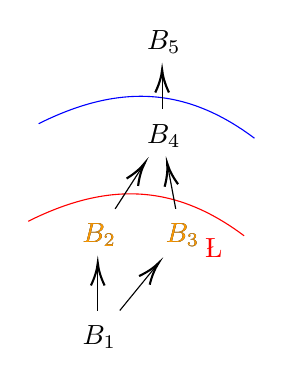
\begin{tikzpicture}[x=0.75pt,y=0.75pt,yscale=-1,xscale=1]
%uncomment if require: \path (0,534); %set diagram left start at 0, and has height of 534

%Curve Lines [id:da3428774655789326] 
\onslide<2->{\draw [color={rgb, 255:red, 255; green, 0; blue, 0 }  ,draw opacity=1 ]   (253,380) .. controls (293,360) and (325,363) .. (357,387) ;}
%Curve Lines [id:da41651271023154823] 
\onslide<2->{\draw [color={rgb, 255:red, 0; green, 0; blue, 255 }  ,draw opacity=1 ]   (258,333) .. controls (298,313) and (330,316) .. (362,340) ;}

% Text Node
\onslide<2-4>{\draw (278,380) node [anchor=north west][inner sep=0.75pt]    {$B_{2}$};}
\onslide<5->{\draw (278,380) node [anchor=north west][inner sep=0.75pt] [color={rgb, 255:red, 250; green, 153; blue, 3 }  ]    {$B_{2}$};}
% Text Node
\onslide<2-3>{\draw (309,332) node [anchor=north west][inner sep=0.75pt]    {$B_{4}$};}
\onslide<4->{\draw (309,332) node [anchor=north west][inner sep=0.75pt] [opacity=0.2  ]    {$B_{4}$};}
% Text Node
\draw (278,429) node [anchor=north west][inner sep=0.75pt]    {$B_{1}$};
% Text Node
\onslide<2-4>{\draw (318,380) node [anchor=north west][inner sep=0.75pt]    {$B_{3}$};}
\onslide<5->{\draw (318,380) node [anchor=north west][inner sep=0.75pt] [color={rgb, 255:red, 250; green, 153; blue, 3 }  ]    {$B_{3}$};}
% Text Node
\onslide<2>{\draw (309,287) node [anchor=north west][inner sep=0.75pt]    {$B_{5}$};}
\onslide<3->{\draw (309,287) node [anchor=north west][inner sep=0.75pt] [opacity=0.2  ]    {$B_{5}$};}

% Connection 1
\draw    (286.5,402) -- (286.5,423) ;
\draw [shift={(286.5,400)}, rotate = 90] [color={rgb, 255:red, 0; green, 0; blue, 0 }  ][line width=0.75]    (10.93,-3.29) .. controls (6.95,-1.4) and (3.31,-0.3) .. (0,0) .. controls (3.31,0.3) and (6.95,1.4) .. (10.93,3.29)   ;
% Connection 3
\onslide<2-3>{\draw    (294.9,374) -- (308.02,353.68) ;
\draw [shift={(309.1,352)}, rotate = 122.86] [color={rgb, 255:red, 0; green, 0; blue, 0 }  ][line width=0.75]    (10.93,-3.29) .. controls (6.95,-1.4) and (3.31,-0.3) .. (0,0) .. controls (3.31,0.3) and (6.95,1.4) .. (10.93,3.29)   ;}
\onslide<4->{\draw [opacity=0.2  ]    (294.9,374) -- (308.02,353.68) ;
\draw [shift={(309.1,352)}, rotate = 122.86] [color={rgb, 255:red, 0; green, 0; blue, 0 },opacity=0.2  ][line width=0.75]    (10.93,-3.29) .. controls (6.95,-1.4) and (3.31,-0.3) .. (0,0) .. controls (3.31,0.3) and (6.95,1.4) .. (10.93,3.29)   ;}
% Connection 4
\onslide<2-3>{\draw    (324.06,374) -- (320.31,353.97) ;
\draw [shift={(319.94,352)}, rotate = 79.38] [color={rgb, 255:red, 0; green, 0; blue, 0 }  ][line width=0.75]    (10.93,-3.29) .. controls (6.95,-1.4) and (3.31,-0.3) .. (0,0) .. controls (3.31,0.3) and (6.95,1.4) .. (10.93,3.29)   ;}
\onslide<4->{\draw [opacity=0.2  ]    (324.06,374) -- (320.31,353.97) ;
\draw [shift={(319.94,352)}, rotate = 79.38] [color={rgb, 255:red, 0; green, 0; blue, 0 },opacity=0.2  ][line width=0.75]    (10.93,-3.29) .. controls (6.95,-1.4) and (3.31,-0.3) .. (0,0) .. controls (3.31,0.3) and (6.95,1.4) .. (10.93,3.29)   ;}
% Connection 2
\draw    (297.11,423) -- (314.62,401.55) ;
\draw [shift={(315.89,400)}, rotate = 129.23] [color={rgb, 255:red, 0; green, 0; blue, 0 }  ][line width=0.75]    (10.93,-3.29) .. controls (6.95,-1.4) and (3.31,-0.3) .. (0,0) .. controls (3.31,0.3) and (6.95,1.4) .. (10.93,3.29)   ;
% Connection 5
\onslide<2>{\draw    (317.5,326) -- (317.5,309) ;
\draw [shift={(317.5,307)}, rotate = 90] [color={rgb, 255:red, 0; green, 0; blue, 0 }  ][line width=0.75]    (10.93,-3.29) .. controls (6.95,-1.4) and (3.31,-0.3) .. (0,0) .. controls (3.31,0.3) and (6.95,1.4) .. (10.93,3.29)   ;}
\onslide<3->{\draw [opacity=0.2  ]    (317.5,326) -- (317.5,309) ;
\draw [shift={(317.5,307)}, rotate = 90] [color={rgb, 255:red, 0; green, 0; blue, 0 },opacity=0.2  ][line width=0.75]    (10.93,-3.29) .. controls (6.95,-1.4) and (3.31,-0.3) .. (0,0) .. controls (3.31,0.3) and (6.95,1.4) .. (10.93,3.29)   ;}

% \draw (250,287) node [anchor=north west][inner sep=0.75pt]    {$G$};

% % Text Node
% \onslide<2->{\draw (228,350) node [anchor=north west][inner sep=0.75pt]  [font=\small,color={rgb, 255:red, 0; green, 0; blue, 0 }  ,opacity=1 ]  {$\tau =\nicefrac{1}{4}$};}

% Text Node
\onslide<2->{\draw (337,387) node [anchor=north west][inner sep=0.75pt]  [color={rgb, 255:red, 255; green, 0; blue, 0 }  ,opacity=1 ]  {$\L$};}
% Text Node
\onslide<2->{\draw (335,338) node [anchor=north west][inner sep=0.75pt]  [color={rgb, 255:red, 0; green, 0; blue, 255 }  ,opacity=1 ]  {$\U$};}

\end{tikzpicture}

% \end{column}
% \begin{column}{0\textwidth}
% \end{column}
% \end{columns}\pause\pause

$\epsW$ is polynomial under common LLL conditions!

% \begin{align*}
%     \sum_{B \in \B} \sum_{\substack{G \in \U \cup \L \\ \text{with sink $B$}}} \only<7>{1}\pause\frac{\epsw(G - B)}{\tau} \pause\leq \frac{1}{\tau} \sum_{B \in \B} \frac{\epsw(\G_B)}{\epslaw(B)}
%                 %  &\pause\eqdef \frac{\epsW}{\tau} \pause\leq \frac{2 \epsW}{\taumax} = 2 \epsW \epsw(\U)^{\nicefrac{1}{\epsilon}} \pause\leq 2 \epsW^{1+\nicefrac{1}{\epsilon}}.% \text{ as $\epsw(\U) \leq \epsW$}.
% \end{align*}
\end{frame}

\subsection{The Algorithm}
\begin{frame}{The Algorithm}
% \r{TODO: $\epsalpha(B)$ for k-SAT}\pause

\begin{algorithm}[H]
\TitleOfAlgo{Deterministic MT-Algorithm}\pause
Using exponential backoff, select ``large'' $\tau$ such that $\w(\U) < 1$\;
% Generate the witness DAGs $\U$\;
Using method of conditional expectations, find resampling table $R$ avoiding $\U$\;
Run the deterministic MT algorithm on $R$\;
\end{algorithm}\spadding

We have seen that the final step takes at most $|\compat{\G}{R}| \leq |\compat{\L}{R}|$ iterations!
\end{frame}

\subsection{Limitations}
\begin{frame}{Limitations}
This algorithm does not cover some scenarios:
\begin{itemize}
    \item superpolynomial $|\B|$ and $|\Sigma|$\pause
    \item non-variable probability spaces\pause
    \item does not cover lopsidependency
\end{itemize}
\end{frame}

% \subsection{Counting Resamples with Witness DAGs}
% \subsubsection{What are Witness DAGs?}
% \begin{frame}{Frame Title}
    
% \end{frame}
% \subsubsection{From Witness DAGs to the Resampling Table to the MT Algorithm}
% \begin{frame}{Frame Title}
    
% \end{frame}
% \subsection{Shearer's Criterion}
% \begin{frame}{Frame Title}
    
% \end{frame}

% \section{A Deterministic Algorithm}
% \begin{frame}{Plan}
% \tableofcontents[currentsection, sectionstyle=show/shaded, hideothersubsections]
% \end{frame}
% \subsection{Shearer's Criterion with Slack}
% \begin{frame}{Frame Title}
    
% \end{frame}
% \subsection{Counting Witness DAGs}
% \begin{frame}{Frame Title}
    
% \end{frame}
% \subsection{Analyzing the Deterministic Algorithm}
% \begin{frame}{Frame Title}
    
% \end{frame}
% \subsection{Pre-processing the Witness DAG and Crisper Results}
% \begin{frame}{Frame Title}
    
% \end{frame}

% \section{Outlook: A Parallel Algorithm and the MT-distribution}
% \begin{frame}{Plan}
% \tableofcontents[currentsection, sectionstyle=show/shaded, hideothersubsections]
% \end{frame}
% \begin{frame}{Frame Title}
    
% \end{frame}

\begin{frame}{}
    \centering \large
    Thanks for your attention!
    Questions?
\end{frame}

\appendix

\begin{frame}{Computing the Resampling Table}
Can $R$ be computed efficiently?\pause\spadding

\underline{Observe}: The MT algorithm uses at most as many columns as the size of the largest witness DAG in $\L$\pause, which is at most $|\L|$.\pause\spadding

For each cell of $R$, choose one of $|\Sigma|$ values to minimize the conditional probability of $G$ \& $R$ being compatible for each $G \in \U$.\pause\spadding

\follows $\O{n |\L| \cdot |\Sigma| \cdot |\L| T \cdot |\U|}$\pause, where $T$ is the runtime of computing conditional probabilities of bad-events given a partial resampling table.\pause\par
Also need to generate $\U$, which can be done in $\poly{|\U|}$ time.
\end{frame}

\begin{frame}{Polynomial Bound of $\nicefrac{\epsw(\G_B)}{\epslaw(B)}$}
$\mu^{(h)}(I) = w(\{G \mid \text{sink $I$, max. depth $h$}\})$ \follows $\mu(B) = w(\G_B)$.\pause\spadding

We have,
\begin{enumerate}
    \item $\mu^{(h+1)}(I) = p(I) \sum_{J \in \text{Stab}(I)} \mu^{(h)}(J)$\pause
    \item $\mu^{(h)}(I) \leq \prod_{B \in I} \mu^{(h)}(B)$ if $\mu(B) \defeq e p(B)$
\end{enumerate}\pause

\begin{align*}
    \mu^{(h+1)}(B) &= p(B) \sum_{J \in \text{Stab}(B)} \mu^{(h)}(J) \\
                   &\leq p(B) \sum_{J \subseteq \bar{\Gamma}(B)} \prod_{B' \in J} \mu^{(h)}(B') \\
    \sum_{J \subseteq \bar{\Gamma}(B)} \prod_{B' \in J} e p(B') &\leq \sum_{J \subseteq \bar{\Gamma}(B)} (e \pmax)^{|J|} \leq \sum_{k=0}^d {d \choose k} (e \pmax)^k \\
    &= (1 + e \pmax)^d \leq \exp(\underbrace{e \pmax d}_{\leq 1}) \leq e.
\end{align*}
\end{frame}

\end{document}